\documentclass[12pt]{report}
\usepackage{graphicx} % Required for inserting images
\linespread{1.2}

\usepackage[dvipsnames]{xcolor}
\usepackage{tikz}
\usepackage[breakable]{tcolorbox}
\appto{\bibsetup}{\raggedright}

\tikzstyle{mybox} = [draw=Dandelion, fill=Dandelion!5, ultra thick, rectangle, rounded corners, inner sep=10pt, inner ysep=15pt, text width=0.90\textwidth, align=left] 
\tikzstyle{boxtitle} = [fill=Dandelion, text=Brown, ultra thick, rectangle, rounded corners, inner sep=10pt, inner ysep=8pt, text width=0.90\textwidth]

\newcommand{\BoxDef}[2]{%
\vspace*{10px}
\noindent

\begin{center}
\begin{tikzpicture}
    \node[mybox](box){\rule{0pt}{30pt}\ignorespaces#2\unskip};
    \node[boxtitle, anchor=north west] at (box.north west) {\textbf{#1}};
\end{tikzpicture}
\end{center}
}

\usepackage[hidelinks]{hyperref}

\usepackage{amsmath}
\usepackage{amssymb}
\usepackage{bm}
\usepackage[top=2.5cm, bottom=2.5cm, left=3cm, right=3cm, centering]{geometry}
\usepackage{algorithm}
\usepackage{algpseudocode}
\usepackage{tabularx}

\begin{document}

\begin{titlepage}
\hrule
\vspace{15pt}
\begin{center}
    \Huge{\textbf{\Huge \textbf{Data Mining 1 23-24}} \\ Notes}\\
\end{center}
\vspace{15pt}
\hrule
\vfill
\hrule
\begin{center}
    \Large University of Pisa \\ M.Sc. in Data Science and Business Informatics
\end{center}
\end{titlepage}

\tableofcontents

\chapter{Data understanding}
This chapter gives an overview of basic terminology and explains some common techniques of data understanding. Data understanding provides general information about the data: allows us to have a view of the different attributes and how they relate to each other, highlights the presence of wrong or missing values, and so on.

\section{What is data?}

A \textbf{dataset} is a collection of data objects (a.k.a. records, samples, points, patterns, etc.).
A \textbf{data object} is a collection of $n$ attributes (a.k.a. variables, fields, features, etc.). The number of attributes in a data object is called its \textbf{dimensionality}.
An \textbf{attribute} is a property or characteristic of an object that can vary, either from one object to another, or from one time to another. 

\section{Types of attribute}

\BoxDef{Categorical (Qualitative)}{
Attributes that can take one of a limited number of values.
\begin{itemize}
    \item \textbf{Nominal}: attribute values belong to a finite domain of names. E.g.: IDs, zip-codes, eye color, gender;

    \item \textbf{Ordinal}: attribute values belong to a finite domain where a meaningful order can be seen. E.g.: scale of hardness of minerals, grades, street number.
\end{itemize}
}

\BoxDef{Numeric (Quantitative)}{
Attributes that represents a measurable quantity.
\begin{itemize}
    \item \textbf{Interval}: values correspond to measures done on a scale of equal sized units; i.e, a unit of measurement exists. E.g.: calendar data, temperature (in °C or °F);

    \item \textbf{Ratio scaled}: values are expressed by specifying by what order of magnitude they are larger/smaller than some unit of measurement. E.g: distances, temperature (in K).
\end{itemize}
}

\BoxDef{Binary attributes}{
Nominal attributes with only 2 possible outcomes.

\begin{itemize}
    \item \textbf{Symmetric binary}: both outcomes are equally important;
    \item \textbf{Asymmetric binary}: one outcome is more important than the other; the former is typically associated with the value 1.
\end{itemize}
}

\BoxDef{Attributes by number of values}{
Attributes can also be classified as:
\begin{itemize}
    \item \textbf{Discrete}: attribute has a finite (or countably infinite) set of values. They are often represented by integer variables;
    
    \item \textbf{Continuous}: attribute has real numbers as values. They are often represented by floating-point variables.
\end{itemize}
}

The type of attribute can be determined by which of the following operations/properties apply:

\begin{table}[h]
    \centering
    \begin{tabular}{l|l}
        (1) Distinctness & $=, \neq$\\
        (2) Order & $<, >$\\
        (3) Differences are meaningful & $+, -$\\
        (4) Ratios are meaningful & $*, /$\\
    \end{tabular}
\end{table}

\textbf{Nominal}: (1)

\textbf{Ordinal}: (1), (2)

\textbf{Interval}: (1), (2), (3)

\textbf{Ratio}: (1), (2), (3), (4)


\section{Types of dataset}

There are many types of datasets. The following list contains the most commonly used, but it's not exhaustive.

\begin{itemize}
    \item \textbf{Record data}: collection of records (i.e., data objects), each of which is a collection of data fields (i.e., attributes). Record data is usually stored in flat files or relational databases.

    Types include: simple record data, data matrix, transaction data, document-
    term matrix

    \item \textbf{Graph-based data}: used to represent actual graphs, or any data where the relationship between objects is relevant.

    \item \textbf{Ordered data}: the objects/attributes have spatio-temporal relationships.

    Types include: sequential transaction data, sequence data, time series data, spatial and spatio-temporal data.
\end{itemize}


\section{Data Quality}

In data mining, preventing data quality issues is near impossible. Instead, the focus is on detecting and correcting data quality issues, and using algorithms that can handle poor data quality. The first step is called data cleaning.

\subsection{Possible issues}

\paragraph{Measurement and data collection errors}
Omitted data-objects or values, or data-objects inappropriately included.

\paragraph{Noise and artifacts}
Noise is the addition of random error to a measurement. Artifacts are errors caused by a deterministic phenomenons.

\paragraph{Outliers}
Data values/objects that are very inconsistent with the rest. They're either caused by mistakes in measurements, or are actual legitimate measurements we may be interested in discovering. Whether they're the former or the latter, it's often useful to detect and eliminate all outliers from the dataset before analyzing the data, since they may skew certain calculations. The process of finding outliers is called \textbf{outlier detection}.

Single outlier attributes can be discovered by using box plots (for numerical attributes), or bar charts (for categorical attributes). Multidimensional attributes are typically discovered (visually) by using scatter plots and parallel coordinates plot, or by using cluster analysis techniques.

\paragraph{Missing values}
Missing values in one or more attributes of an object. The values may not have been collected to begin with, either because the user chose or forgot to input the data or because a sensor receiving the data broke, or they are intentionally left blank in some objects because they don't apply to those specific objects. Missing values are also not always explicitly indicated as such, and may instead be displayed as a default value or a 0.

\paragraph{Inconsistent data}
Inconsistency regarding either syntax (a value does not appear in the domain of that attribute), or semantic (the value is acceptable, but does not make sense when paired with the other attribute values of the same object).

\paragraph{Duplicate data}
Two or more objects are duplicates of each other. Can be caused by an input mistake, or can be legitimate values that just happen to be identical between objects.

\paragraph{Timeliness}
Data is not up to date.

\paragraph{Unbalanced data}
The dataset is heavily biased towards a certain type of object.

\section{Measures}

\subsection{Measuring the central tendency}

\BoxDef{Mean}{
The mean of a set of values is calculated as:
\begin{equation*}
    mean(x) = \dfrac{1}{m} \sum_{i=1}^{m} x_i
\end{equation*}
}

\BoxDef{Median}{
The median of a set of values is the middle value if the number of elements is odd, else it's the average of the two middle values.
}

\BoxDef{Mode}{
The mode of a set of values is the value with the highest frequency. There may be multiple values with the same (highest) frequency; those are called bimodal, trimodal, ..., multimodal distributions. In case all values have the same frequency, then there is no mode.
}

\subsection{Measuring the dispersion}
The degree in which the data tends to spread is called the \textbf{dispersion}, or \textbf{variance}.

\BoxDef{Variance}{
Variance is calculated as:
\begin{equation*}
    var(x) = \sigma_x^2(x) = \dfrac{\sum_{i=1}^m (x - mean(x))^2}{m-1}
\end{equation*}
}

\BoxDef{Covariance}{
Covariance measures the join variability of two variables, showing how much the two variables are connected by a linear relationship. It's calculated as: 

\begin{equation*}
    cov = \dfrac{\sum_{i=1}^n (x_i - mean(x))(y_i - mean(y))}{n-1}
\end{equation*}

}

\BoxDef{Standard deviation}{
The standard deviation, $\sigma_x$, is calculated as:

\begin{equation*}
    \sigma_x = \sqrt{\sigma_x^2}
\end{equation*}

It measures how much the data spreads w.r.t the mean, so it should be used only when the mean is chosen as the measure of the center. When $\sigma = 0$, all the values are equal (i.e. there is no spread from the mean). When $\sigma > 0$, then there is spread.
}

\BoxDef{Range}{
It's the distance between the largest and the smallest values.
}

\section{Data visualization}

Visualizing data can be an useful and intuitive way to analyze it and detect general trends and patterns (including outliers).

\paragraph{Bar charts and histograms}

A \textbf{bar chart} is used to depict the frequency of \textbf{categorical} attributes. An \textbf{histogram} is used to depict the frequency of \textbf{numerical} attributes. The range of attributes is normally discretized into a fixed number of intervals, called \textbf{bins}.

\begin{figure}[h]
    \centering
    \begin{minipage}[b]{0.40\textwidth}
        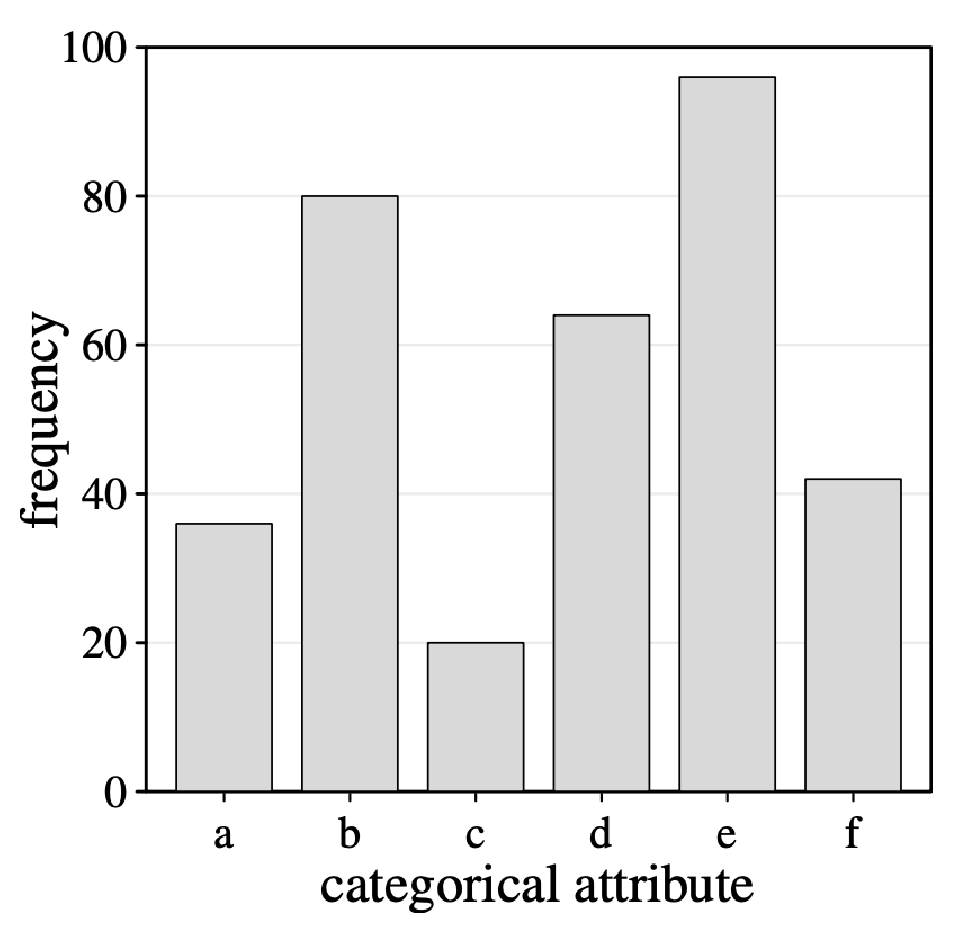
\includegraphics[width=\textwidth]{img/bar chart.png}
        \caption{A bar chart.}
    \end{minipage}
    \hfill
    \begin{minipage}[b]{0.45\textwidth}
        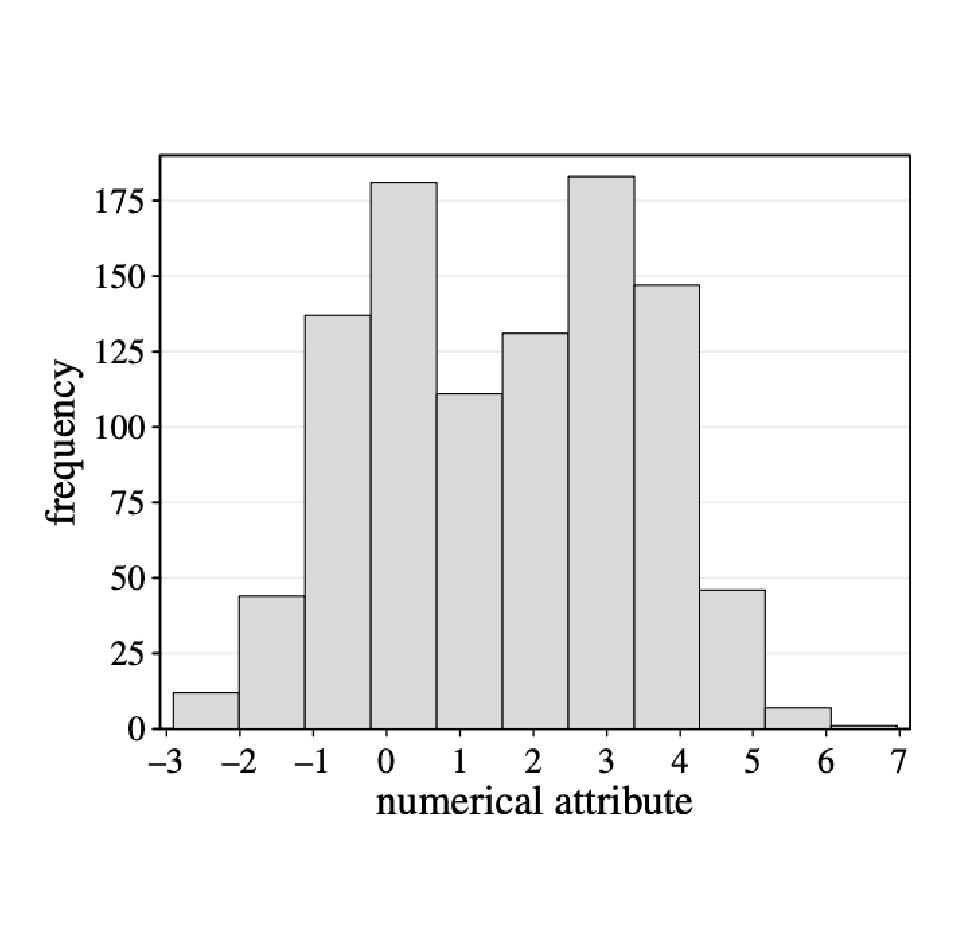
\includegraphics[width=\textwidth]{img/histogram.png}
        \caption{An histogram.}
    \end{minipage}
\end{figure}

\BoxDef{Sturges' rule}{
The number of bins, $k$, can be calculated using Sturges' rule:
\begin{equation*}
    k=\lceil{\log_2(n) + 1}\rceil
\end{equation*}
where $n$ is the number of data objects. This formula is especially suitable for data from normal distributions and from datasets of moderate size.
}

\BoxDef{Natural binning}{
A simple way of distributing values across bins is by using natural binning. Given $\delta$:
\begin{equation*}
    \delta = \dfrac{x_{max} - x_{min}}{k}    
\end{equation*}
then, element $x_j$ belongs to class $i$ if:
\begin{equation*}
    x_j \in [x_{min} + i*\delta, x_{min} + (i+1)*\delta]
\end{equation*}
}

\BoxDef{Equal frequency binning}{
Natural binning can generate an unbalanced distribution, where some bins may contain a lot more elements than others. The alternative is to calculate the frequency, $f$:
\begin{equation*}
    f = \dfrac{N}{k}
\end{equation*}
which determines how many elements must be contained in a single bin. Then, element $x_j$ belongs to class $i$ if:
\begin{equation*}
    i*f \leq j < (i+1)*f
\end{equation*}
}
This last method is not too useful to uncover interesting distribution of data, however.

\paragraph{Scatter plot}
A scatter plot is used to analyze the presence of clusters of points, outliers, and correlation between data points. Each pair of values plotted is treated as a pair of point coordinates that determine where the point will be displayed relative to the $x$ and $y$ axes. Scatter plots may be used to visualize data up to 3 dimensions, where each point has three coordinates, as to visualize three features at once.

Multiple scatter plots can be aggregated in a \textbf{scatter matrix} that combines multiple attributes at once.

\begin{figure}[h]
    \centering
    \begin{minipage}[b]{0.45\textwidth}
        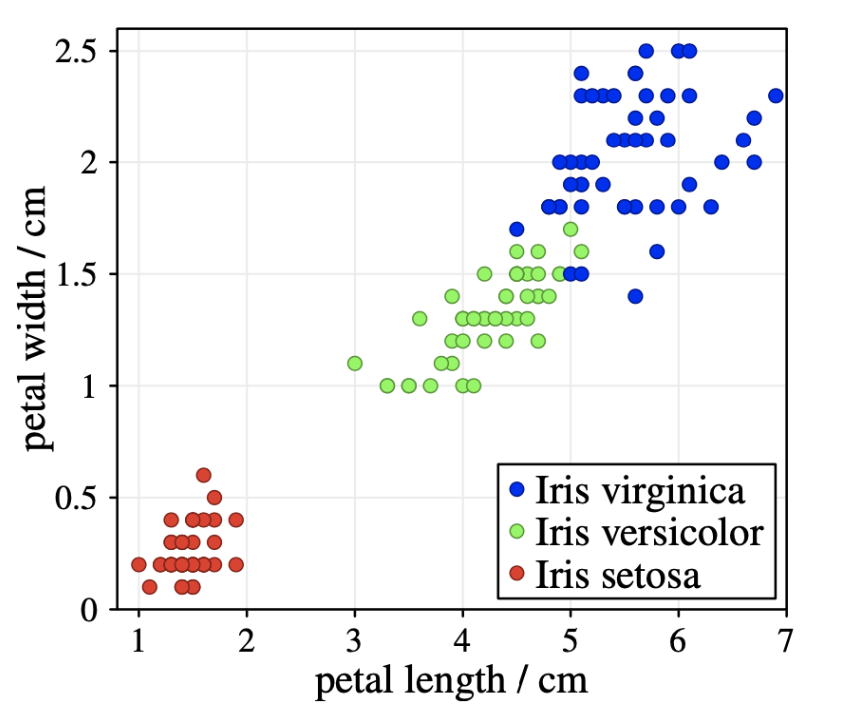
\includegraphics[width=\textwidth]{img/scatter plot.png}
        \caption{A scatter plot.}
    \end{minipage}
    \hfill
    \begin{minipage}[b]{0.47\textwidth}
        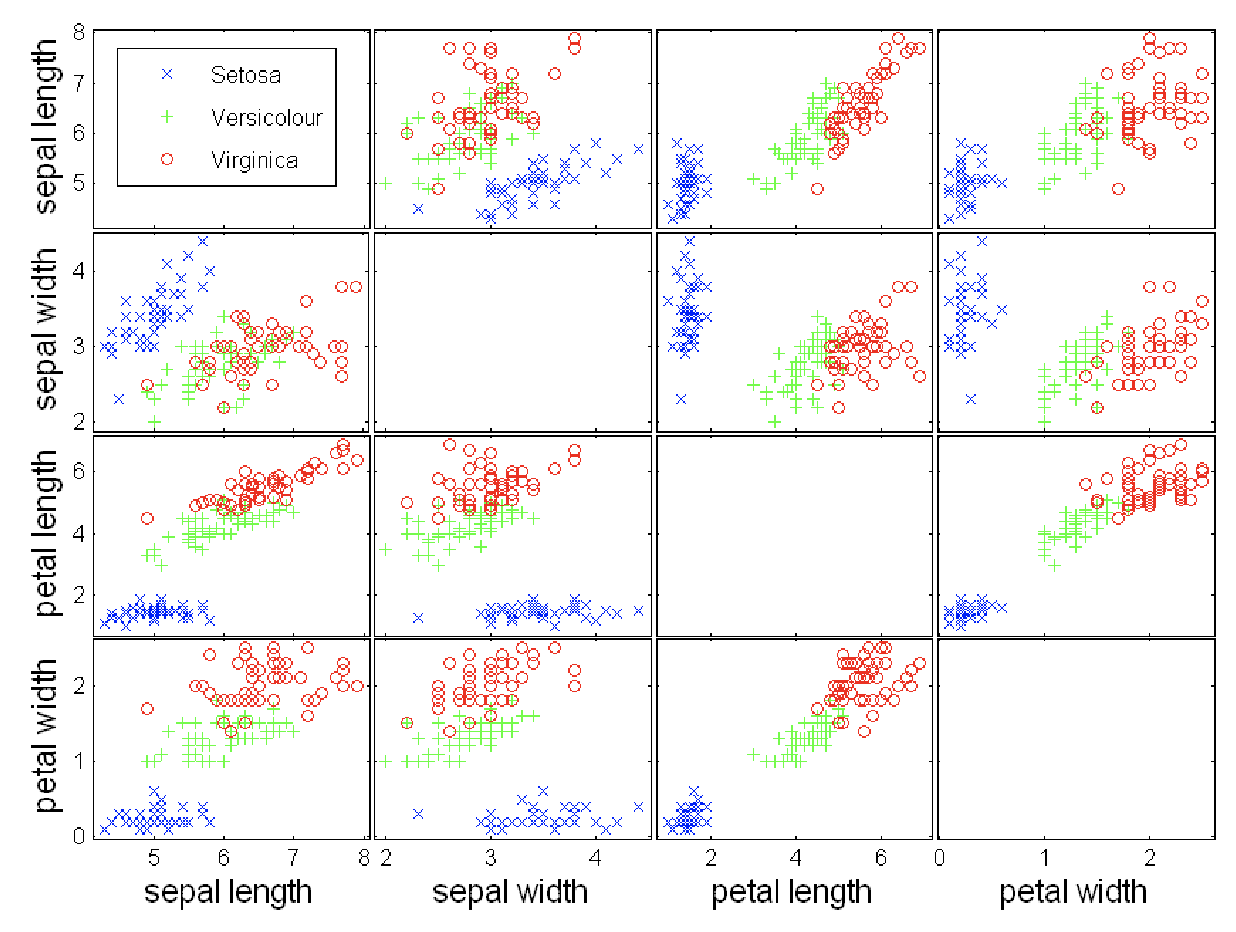
\includegraphics[width=\textwidth]{img/scatter matrix.png}
        \caption{A scatter matrix visualizing multiple scatter plots at once.}
    \end{minipage}
\end{figure}

\paragraph{Five-number summary and box plot}
A five number summary is done by determining five values, typically corresponding to:

\begin{itemize}
    \item $10^{th}$ percentile;
    \item $25^{th}$ percentile (or $1^{st}$ quartile);
    \item $50^{th}$ percentile (or $2^{nd}$ quartile, corresponding to the mean);
    \item $75^{th}$ percentile (or $3^{rd}$ quartile);
    \item $90^{th}$ percentile.
\end{itemize}

Once these values are calculated, the data can be visualized with a \textbf{box plot}. The $25^th$ and $75^{th}$ percentiles are the ends of the box, and the distance between the two is called the \textbf{interquartile range (IQR)}. The $10^{th}$ and $90^{th}$ percentile are instead called \textbf{whiskers}. This way of visualizing data is especially useful for discovering outliers.

\begin{figure}[h]
    \centering
    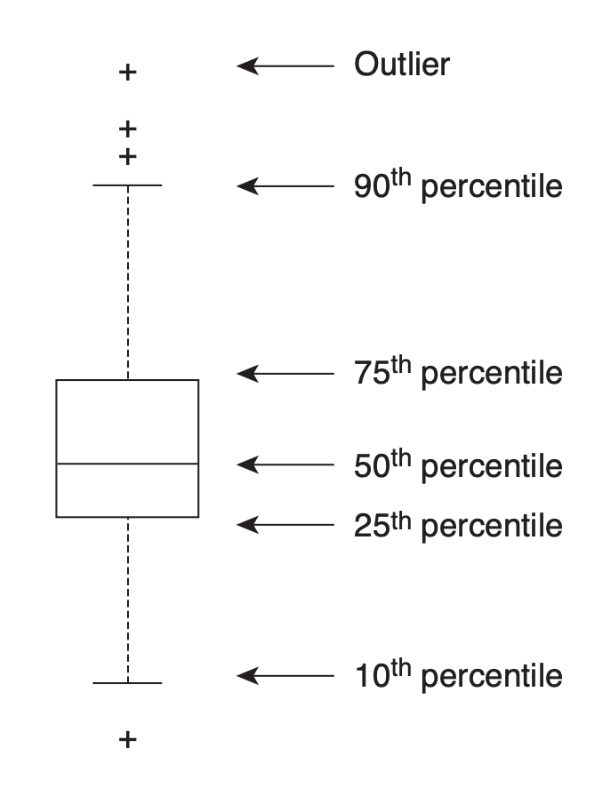
\includegraphics[width=0.4\linewidth]{img/box plot.png}
    \caption{A box plot.}
\end{figure}

\paragraph{Parallel coordinates plot}
This type of plot is often used to visualize attributes of high-dimensional data ($> 3$). Instead of using two perpendicular axes, this plot uses $n$ parallel axes (where $n$ is the number of attributes we want to visualize). The attribute values of each individual object are then plotted as points on each axis, forming a straight line. The resulting plot will contain a separate line for each object in the dataset. Areas with a denser number of lines suggest some correlation between the objects corresponding to those lines.

\begin{figure}[h]
    \centering
    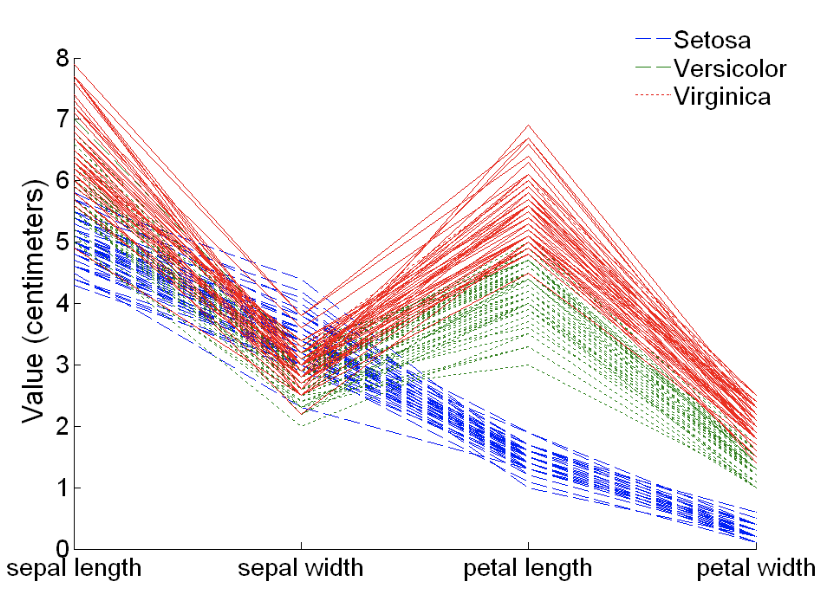
\includegraphics[width=0.4\linewidth]{img/Parallel coord plot.png}  
    \caption{A parallel coordinates plot.}
\end{figure}

\paragraph{Data matrix plot}
Matrix plots are useful to visualize data sorted according to class. The attribute values are normalized to prevent one attribute from dominating the plot. A common type of data matrix plot is the distance matrix, which visualizes the value of the standard deviation $\sigma$ for each value.

\begin{figure}[h]
    \centering
    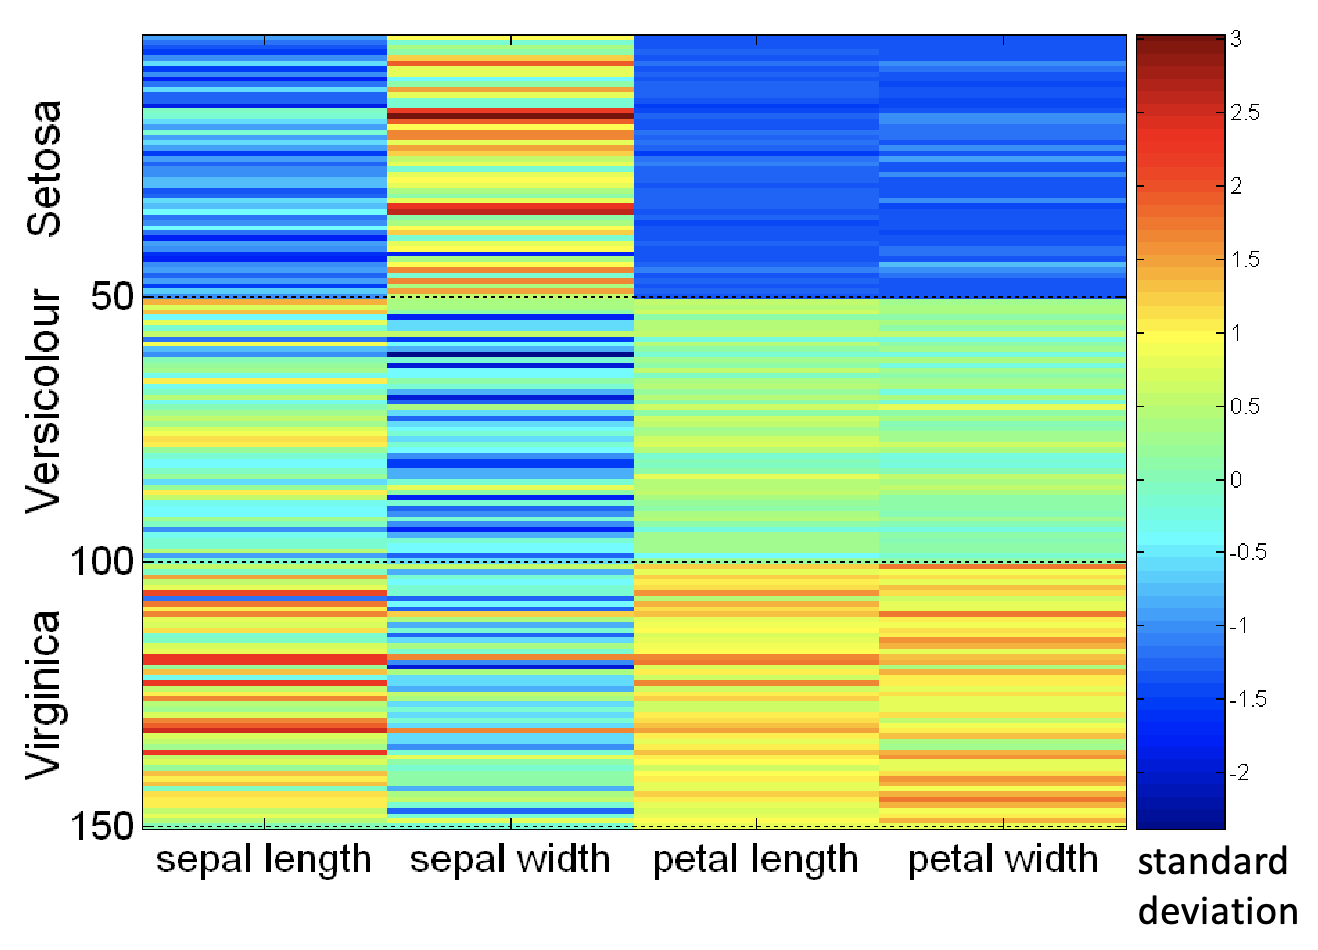
\includegraphics[width=0.4\linewidth]{img/distance matrix.png}
    \caption{A distance matrix plot.}
\end{figure}

\paragraph{Radar plot}
A radar plot is similar to a parallel coordinates plot, in that it uses $n$ different axes, one for each attribute, but instead of placing them in a parallel line, they radiate from a central point. All the lines representing the same object will end up forming a polygon.

\paragraph{Star plot}
The same as radar plots, but points are all drawn separately.

\begin{figure}[h]
    \centering
    \begin{minipage}[b]{0.43\textwidth}
        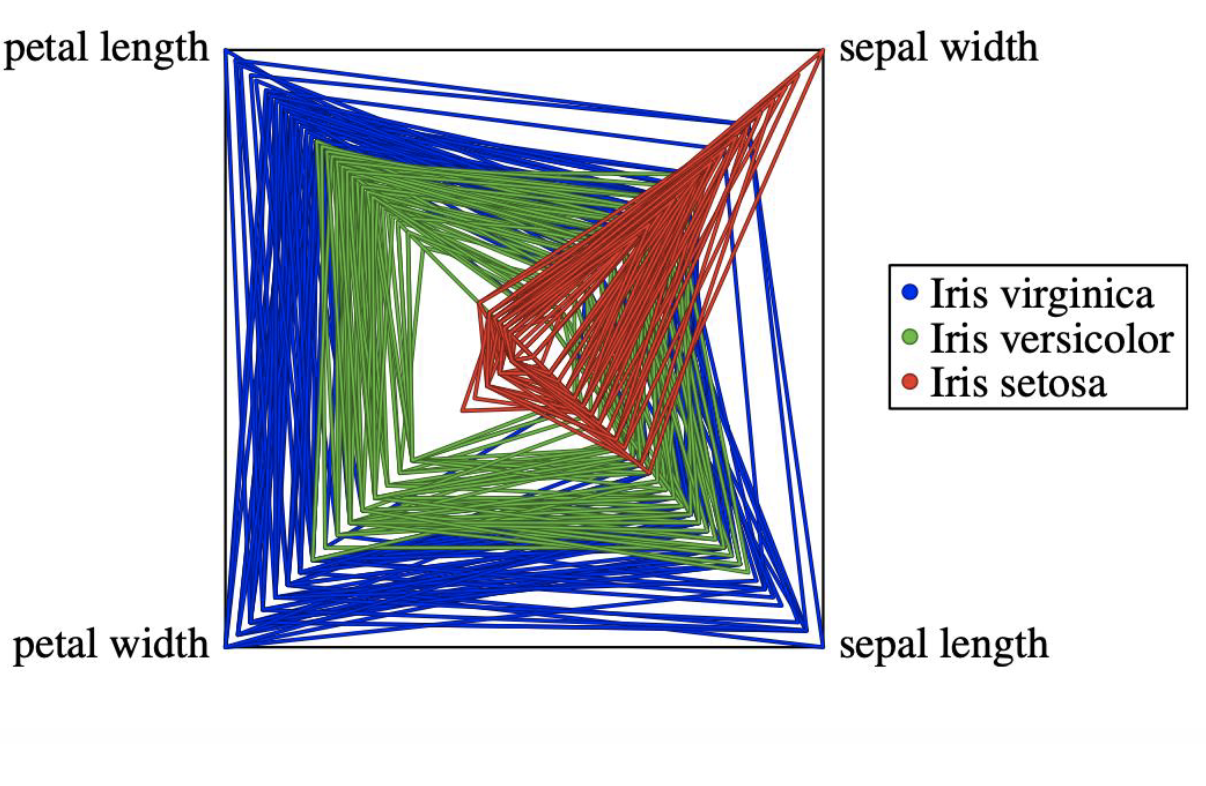
\includegraphics[width=\textwidth]{img/radar plot.png}
        \caption{A radar plot.}
    \end{minipage}
    \hfill
    \begin{minipage}[b]{0.43\textwidth}
        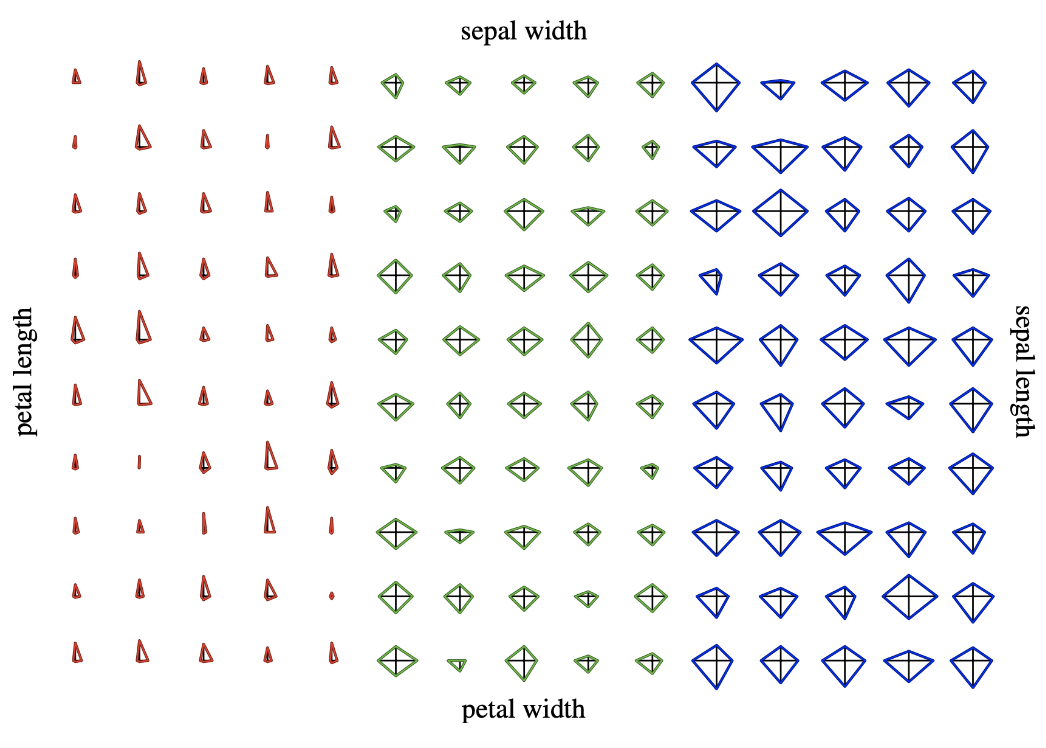
\includegraphics[width=\textwidth]{img/star plot.png}
        \caption{A star plot.}
    \end{minipage}
\end{figure}

\newpage

\section{Correlation analysis}

Correlation analysis is a popular technique for analyzing relationships between pairs of variables. For continuous variables, correlation is defined using \textbf{Pearson's correlation coefficient}.

\BoxDef{Pearson's correlation coefficient}{
Pearson's correlation coefficient between two variables is calculated as:
    \begin{equation*}
        corr(x,y) = \dfrac{cov(x,y)}{\sigma(x) \sigma(y)} = \dfrac{\sum_{i=1}^n (x_i - mean(x))(y_i - mean(y))}{(n-1) \sigma(x) \sigma(y)}
    \end{equation*}
}

The value of this coefficient lays between -1 and 1. When $corr(x,y) = 1$, the two variables have a perfect positive correlation, else if $corr(x,y) = -1$, the two variables have perfect negative correlation. Correlation can also be graphically visualized by using an appropriate plot, called \textbf{correlation matrix}.

\begin{figure}[h]
    \centering
    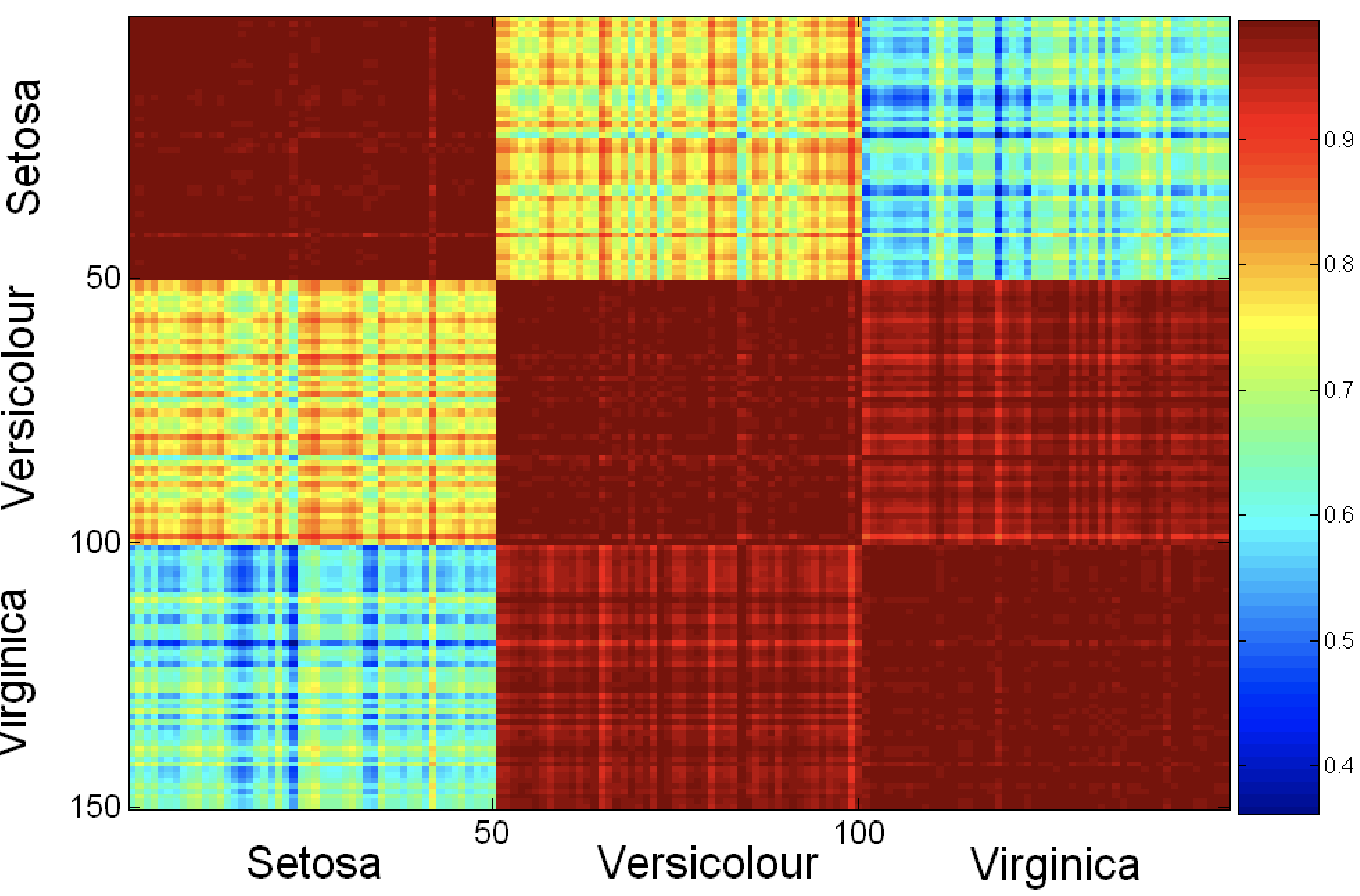
\includegraphics[width=0.4\linewidth]{img/correlation matrix.png}
    \caption{A correlation matrix.}
\end{figure}
\chapter{Data preparation}

Data preparation uses the information provided by data understanding to select attributes, reduce the data dimension, treat missing values and outliers, transform the data and improve its quality.

\section{Overview of techniques}

Roughly speaking, the following topics can be organized in two categories: selectiong data objects and attributes, and creating and changing the attributes.

\subsection{Aggregation}

Aggregation consists in combining two or more objects into a single object. Typically, quantitative attributes are aggregated by taking a sum or an average, while qualitative ones are either omitted or summarized as an higher level category.

There are several motivations for aggregation:

\begin{itemize}
    \item \textbf{Data reduction}: the smaller the size of the dataset, the less memory and processing time it will require;

    \item \textbf{Change of scope or scale}: it can provide a more higher-level view of the data;

    \item \textbf{Stabilizing the data}: the behaviour of groups of objects or attributes is often more stable than that of individual ones. 
\end{itemize}

\subsection{Sampling}

Sampling is commonly used to select a subset of the data objects to be analyzed. The key principle for effective sampling is the following: using a sample will work almost as well as using the entire dataset if the sample is representative.

\paragraph{Representative sample} A sample is representative if it has approximately the same property (of interest) as the original set of data.

There are many sampling techniques:

\begin{itemize}
    \item \textbf{Simple random sampling}: there is an equal probability of selecting any particular object. There's two variations; \textbf{sampling without replacement}, where as each object is selected, it is removed from the set of all objects that constitute the population, and \textbf{sampling with replacement}, where objects are not removed as they are selected, so the same object may be picked more than once.

    \item \textbf{Stratified sampling}: when the population consists of different types of objects, simple random sampling may fail to represent less frequent ones. Stratified sampling starts by using data already organized into groups, and picks an equal number of objects from each group, so that they can all be equally represented.
\end{itemize}

Determining the sample size can be difficult sometimes, so adaptive or \textbf{progressive sampling} schemes are used: these approaches start with a small sample, and increase its size until it's big enough for the task.

\subsection{Dimensionality reduction}

Datasets can have a large number of features, some of which may actually be removed entirely from the dataset without damaging the properties of the data. The reason behind wanting to reduce the dimensionality of data is that it can remove useless attributes, and also remove noise (see: curse of dimensionality; the higher the number of dimensions, the sparser the data) and make the data easier to visualize. Another obvious advantage is a reduction in actual memory required to store the dataset.

The main techniques of dimensionality reduction include:

\begin{itemize}
    \item \textbf{Principal Components Analysis (PCA)}: a linear algebra technique that finds new attributes that are linear combinations of the original attributes, orthogonal to each other, and capture the maximum amount of variation in the data.

    \item \textbf{Singular Value Decomposition (SVD)}: a linear algebra technique that is related to PCA.
\end{itemize}

\subsubsection{PCA}
Variance and covariance are key factors in constructing PCA. \textbf{Variance} measures the spread of a set of points from the mean, while \textbf{covariance} is a measure of how much each of the dimensions vary from the mean with respect to each other. SO, covariance is measured between two dimensions to see if there's a relationship. The covariance between a dimension and itself is the variance.

The first principal component is the dimension with the largest possible variance in the dataset. The second principal one is calculated in the same way, with the condition that it is uncorrelated with the first principal component and also accounts for the next highest variance.

\subsection{Feature subsection selection}

Another way of reducing the dimensionality of the dataset is to only select a subset of the features; this technique is used in the presence of redundant features and irrelevant features. \textbf{Redundant features} duplicate much or all information contained in one or more attributes. \textbf{Irrelevant features} contain almost to no useful information for the task at hand.

While some irrelevant or redundant features can be removed by simply using commons sense or domain knowledge, sometimes a more systematic approach is needed. The simplest approach is to try all possible subsets of features as input to the algorithm we want to use, and take the one that produces the best output. However, the number of subsets involving $n$ attributes would be $2^n$, so this approach is often very impractical. There are three standard approaches used for feature selection, explained below.

\begin{itemize}
    \item \textbf{Embedded approaches}: feature selection occurs naturally as part of the data mining algorithm. Specifically, it's the algorithm itself that selects which attributes to use and which to ignore. 

    \item \textbf{Filter approaches}: features are selected before the algorithm is run, using an approach independent from the task that uses the significance and correlation between attributes to do the selection.

    \item \textbf{Wrapper approaches}: these methods use the target data mining algorithm as a black box o find the best subset, similarly to the brute-force approach described above, but without enumerating all subsets. Some techniques include selecting the top-ranked features, selecting the top ranked subset, forward selection (starting with an empty subset, add one feature at a time, then yield the one with the best improvement), backward elimination (start with the full set of features, remove one by one, remove completely the one the yields the least decrease in performance).
\end{itemize}

\subsection{Feature creation}

It's also possible to create new features starting from existing ones that are capable of capturing the important information better. The final number of attributes can be smaller than the starting one, reducing the dimensionality as well. There are two general methodologies to do feature creation:

\begin{itemize}
    \item \textbf{Feature construction/extraction}: the new higher-level features are created by combining the original features. This is a highly domain-specific technique. An example of feature construction may be the following: a dataset where each object has attributes \textit{mass} and \textit{volume}, we can combine them to construct the attribute \textit{density = mass / volume}, and remove the previous two attributes.

    \item \textbf{Feature projection}: the data is mapped to a new space with lower dimensionality. This mapping may be linear or nonlinear, and can be achieved with many approaches, such as PCA, SVD, non-negative matrix factorization (NMF), linear discrimination analysis (LDA), and autoencoders.
\end{itemize}

\subsection{Data cleaning}

Data cleaning involves handling of anomalous values and outliers. \textbf{Missing values} are values that were not inserted into the dataset, whether because the user refused to give certain information, or because a sensor or other system to collect data was malfunctioning. They're often marked by a special value, commonly \textit{NULL} or $?$, but may also correspond to a default value (and be much more difficult to recognize as a result). \textbf{Unknown values} are values without a real meaning. \textbf{Invalid values} are values that are not significant to the task.

In order to manage missing values, the two approaches are:

\begin{itemize}
    \item \textbf{Eliminating records}: the whole record is removed (removing all the other attribute values);

    \item \textbf{Substitution of values}: the missing values can be replaced by the mean / median / mode, or by an estimate made using the probability distribution of existing values.
\end{itemize}

\subsection{Discretization and binarization}

Some algorithms may specifically require that the data be in the form of categorical attributes. If the dataset presents continuous attributes, it may be necessary to transform them into discrete ones (\textbf{discretization}), or to transform them into one or more binary attributes (\textbf{binarization}). The ideal discretization or binarization approach would need to know the probability distribution of the data, which more often than not in unknown.

Discretization is often used for attributes that are used in classification or association analysis. Transformation of a continuous attribute to a categorical one can be divided into two tasks: in the first one, the values of that attribute are sorted and divided into $n$ intervals by specifying $n-1$ split points; in the second step, all the values of one interval are mapped to the same categorical value. The problem consists in deciding how many split points to insert, and where to place them.
\begin{itemize}
    \item \textbf{Unsupervised discretization}: class information is not used: there's no labels for the instances, and the number of overall classes is unknown. The most common approaches are \textbf{natural binning}, \textbf{equal frequency binning}, and \textbf{statistical binning}.

    If the number of final groups is too little, there is loss of information; if it's too high, there's too much dispersion in the data. The optimal number of classes to divide $N$ elements can be calculated as:

    \begin{equation*}
        C = 1 + \dfrac{10}{3}\log_{10}(N)
    \end{equation*}

    and the optimal width of the classes:

    \begin{equation*}
        h = \dfrac{3.5 s}{\sqrt{N}}
    \end{equation*}

    \item \textbf{Supervised discretization}: class information is known. The most common approaches are \textbf{entropy-based}, and \textbf{based on percentiles}.
\end{itemize}

Binarization is often used for association analysis tasks. A simple technique to binarize a categorical attribute is the following: if there are $m$ categorical values, assign each value to an integer  in the interval $[0, m-1]$. If the attribute is ordinal, order must be maintained by the assignment. Next, convert each of these $m$ integers to binary values: since $n = \lceil \log_2(m) \rceil$ binary digits are used to represent these integers, represent these binary numbers using $n$ new binary attributes.

\subsection{Attribute/Variable transformation}

An attribute transformation refers to a transformation applied to all the values of an attribute. Some common transformations include:

\begin{itemize}
    \item \textbf{Simple functions}: $x^k$, $\log (x)$, $e^x$, $\sqrt{x}$, $\frac{1}{x}$, $\sin{x}$, etc.;

    \item \textbf{Normalization or standardization}: a set of techniques used to adjust the differences among attributes in terms of frequency of occurrence, mean, variance and range.
\end{itemize}

A \textbf{transformation T} on the attribute $X$ is defined as: $Y = T(x)$, such that $Y$ preserves the relevant information of $X$, eliminates at least one of the problems of $X$, and is more useful than $X$.

Some common normalizations are \textbf{min-max normalization} and \textbf{z-score normalization}.

\BoxDef{Min-Max normalization (rescaling)}{
\begin{equation*}
    v' = \dfrac{v-min_A}{max_A - min_A} (new\_max_A - new\_min_A) + new\_min_A
\end{equation*}
}

\BoxDef{Z-score normalization (standardization)}{
\begin{equation*}
    v' = \dfrac{v-mean_A}{\sigma_A}
\end{equation*}
}

A common transformation function is the \textbf{exponential transformation}:

\begin{equation*}
    T_p(x) = \begin{cases}
                ax^p+ b & p \neq 0 \\
                c\log x + d & p = 0
            \end{cases}   
\end{equation*}

with $a$, $b$, $c$, $d$, $p$ real values.
\chapter{Data similarity}

Similarity and dissimilarity are important because they are used for many data mining techniques, such as clustering, nn classification, and anomaly detection.

\textbf{Similarity} is a numerical measure of how alike two data objects are: the higher the similarity, the more they are alike. It often falls in the range $[0,1]$.

\textbf{Dissimilarity} is a numerical measure of how different two data objects are: the higher the dissimilarity, the more they are different. The minimum value is often $0$, while the upper limit varies.

The term \textbf{proximity} is used to refer to either similarity or dissimilarity.

\section{Similarity and dissimilarity between attributes}

The proximity of objects is often measured by combining the proximities of their single attributes, so we first discuss how proximity is calculated across the same attribute.
The following table sums up how proximity is calculated for nominal, ordinal and interval or ratio attributes.

\begin{table}[h]
    \centering
    \begin{tabular}{c|c|c}
        Type & Dissimilarity & Similarity \\
        \hline
        Nominal & $d=\begin{cases}
                    0 & x = y \\
                    1 & x \neq y
                    \end{cases}$ & $s=\begin{cases}
                    0 & x \neq y \\
                    1 & x = y
                    \end{cases}$ \\
        \hline
        Ordinal & $d = \dfrac{|x-y|}{(n-1)}$ & $s = 1-d$\\
        \hline
        Interval or Ratio & $d = |x - y|$ & $s = -d$, $s=\frac{1}{1+d}$, $s = e^{-d}$\\
    \end{tabular}
\end{table}

\section{Similarity and dissimilarity between data objects}

\subsection{Dissimilarity}
Dissimilarity between data objects are often calculated using distances, which are a kind of dissimilarities with certain propertites.

\BoxDef{Minkowski distance}{
The Minkowski distance between two points $x$ and $y$ is calculated as:
\begin{equation*}
    d(x,y) = (\sum_{k=1}^n |x_k - y_k|^r)^{\frac{1}{r}}
\end{equation*}
}

The following are the three most common examples of Minkowski distances:

\begin{itemize}
    \item \textbf{Manhattan distance}: r=1
    \item \textbf{Euclidean distance}: r=2
    \item \textbf{Supremum distance}: r=$\inf$
\end{itemize}

\paragraph{Properties of distances}

\begin{itemize}
    \item \textbf{Positivity}
    
    $d(x,y) \geq 0 \forall x,y$; $d(x,y) = 0$ only if $x = y$;

    \item \textbf{Symmetry}

    $d(x,y) = d(y,x) \forall x,y$;

    \item \textbf{Triangle inequality}

    $d(x,z) \leq d(x,y) + d(y,z) \forall x,y,z$.
\end{itemize}
Measures that satisfy all three properties are called \textbf{metrics}.

\subsection{Similarities}

For similarities, the triangle inequality typically does not hold, but symmetry and positivity usually do.

\paragraph{Properties of similarities}

\begin{itemize}
    \item \textbf{Positivity}

    $0 \leq s(x,y) \leq 1 \forall x,y$; $s(x,y) = 1$ only if $x=y$;

    \item \textbf{Symmetry}

    $s(x,y) = s(y,x) \forall x,y$
\end{itemize}

\subsection{Similarity between binary vectors}
Similarity measures between objects that contain only binary attributes are called \textbf{similarity coefficients}, and typically have values between 0 and 1.

Let $x$ and $y$ be two objects that consist of $n$ binary attributes. The comparison between these two objects leads to the following four quantities:

$f_{00}$ = the number of attributes where $x = 0$ and $y = 0$

$f_{01}$ = the number of attributes where $x = 0$ and $y = 1$

$f_{10}$ = the number of attributes where $x = 1$ and $y = 0$

$f_{11}$ = the number of attributes where $x = 1$ and $y = 1$

We can then define two ways to measure similarity:

\BoxDef{Simple Matching Coefficient (SMC)}{
    \begin{equation*}
        SMC = \dfrac{f_{11} + f_{00}}{f_{00} + f_{01} + f_{10} + f_{11}}
    \end{equation*}
}
This measure counts both presences and absences equally.

\BoxDef{Jaccard coefficient}{
    \begin{equation*}
        J = \dfrac{f_{11}}{f_{01} + f_{10} + f_{11}}
    \end{equation*}
}    
This measure considers presences only.

\BoxDef{Cosine Similarity}{
\begin{equation*}
    cos(x,y) = \dfrac{\langle x,y \rangle}{\|x\|_2\|y\|_2} = \dfrac{x^T y}{\|x\|_2\|y\|_2}
\end{equation*}
}
This similarity is often used for document vectors, where very few attributes per vector are non-zero and thus the similarity between the documents should not consider the number of shared 0s; the reason Jaccard distance isn't used is that it can't handle non binary attributes.

\section{Correlation}

Correlation measures the linear relationship between two sets of values that are observed together. It can measure the relationship between both attributes and data objects. There are many types of correlation; a measure appropriate for numerical values is Pearson's correlation.

How to deal with data that has both continuous and categorical attributes? The first option is to simply pretend that categorical attributes can be represented as values and use continuous distances (obviously not the right one). The second option is to discretize the continuous attributes and use categorical distances (Jaccard, cosine, SMC).

The third option is to define a new heterogeneous distance as:

\begin{equation*}
    d(x,y) = \frac{n_{cat}}{n} d_{cat}(x_{cat}, y_{cat}) + \frac{n_{con}}{n} d_{con}(x_{con},y_{con})
\end{equation*}
\chapter{Clustering}

Cluster analysis groups data objects into clusters based on the information found in the data itself. The goal is to produce clusters such that all of the members of a single cluster are similar to each other, while objects belonging to different clusters are unrelated.

The main reasons behind clustering analysis are:

\begin{itemize}
    \item \textbf{Understanding}: identifying classes and groups of objects plays an important role in how people analyze the world. Humans are naturally efficient at finding clusters and classifying new data on the basis of the clusters found. Cluster analysis is also often referred to as \textbf{unsupervised classification} for this reason (as opposed to classic classification, which is supervised).

    \item \textbf{Summarization}: if instead of applying an algorithm to the whole dataset, it is applied to (accurately defined) clusters, the efficiency of the excution may be increased. This is especially important for algorithms that have a complexity of $O(l^2)$, such as regression or component analysis.
\end{itemize}

\section{Types of clusterings}

Clusterings are a collection of clusters.

\begin{itemize}
    \item \textbf{Hierarchical vs Partitional}: this is the most commonly discussed partitioning. A \textbf{partitional clustering} is a division of the dataset into non overlapping clusters (i.e., the intersection of each pair of clusters is $\empty$). \textbf{Hierarchical clustering} finds a set of nested clusters that form a hierarchy organized as a tree. The cluster at the root is the cluster that contains all the others.

    \item \textbf{Exclusive vs Overlapping vs Fuzzy}: an \textbf{exclusive clustering} assigns each object to only one cluster. \textbf{Overlapping (or non-exclusive) clustering} may assign on object to multiple clusters at once. in \textbf{fuzzy clustering}, every object belongs to every cluster with a weight between 0 and 1 that measures "how much" that object belongs to a given cluster: a weight of 0 means it absolutely doesn't belong, while 1 means that it absolutely belong. The sum of all the weights of a data object must sum to 1.

    \item \textbf{Complete vs Partial}: a \textbf{complete clustering} assigns each object to a cluster, while a \textbf{partial clustering} does not; typically, it excludes noise and outliers that may erroneously influence the properties of the clusters during further analysis.

    \item \textbf{Heterogeneous vs Homogeneous}: in \textbf{heterogeneous clustering}, all clusters have the same size/shape/density, while in \textbf{Homogeneous clustering} the cluster may differ.
\end{itemize}

\section{Types of clusters}

\begin{itemize}
    \item \textbf{Well separated}: a cluster is a set of objects in which each object is closer (or more similar) to any other point in its cluster than to any point belonging to a different cluster. This idealistic definition of cluster is satisfied only when the data contains natual clusters that are all far apart from each other. These clusters can have any shape.

    \item \textbf{Prototype-based and center-based}: a cluster is a set of objects in which each object is closer to the prototype that defines the cluster it belongs to than to any other prototype. For data with continuous attributes, the prototype is often a \textbf{centroid}, calculated as the mean of all points. If the centroid is not meaningful, for example if the attributes are categorical, a \textbf{medoid} is used instead; which is the most representative point in the cluster. For many types of data, the prototype is also the most central point; we refer to these clusters as \textbf{center-based clusters}.

    \item \textbf{Graph-based}: if the data can be represented by a graph, where the nodes are the objects and the links represent connections between objects, than a cluster can be defined as a \textbf{connected component}. An important type of graph-based clusters is a \textbf{contiguity-based cluster}, where two objects are connected only if they are in a specified distance from each other: each point is closer to just one other point in the cluster than it is closer to any other point in a different cluster. This definition is useful for clusters that are very irregular and intertwined.
    
    \item \textbf{Density-based}: a cluster is a dense region of objects that is surrounded by a region of low density. This definition is also useful for irregular clusters.

    \item \textbf{Shared-property (or Conceptual clusters)}: a cluster is defined as a set of objects that share a generic property. This definition encompasses all the previous ones, and includes new ones.

    \item \textbf{Objective function}: clusters are found so that they minimize or maximize an objective function.
\end{itemize}

\section{K-means}

K-means clustering is a technique that defines prototypes in terms of centroids, which are the mean of a group of points.

\begin{algorithm}
\caption{Basic K-means algorithm.}
\begin{algorithmic}[1]
    \State Select K points as initial centroids.

    \Repeat
        \State Form K clusters by assigning each point to its closest centroid.

        \State Recompute centroids of each cluster.
    \Until{Centroids do not change.}
\end{algorithmic}
\end{algorithm}

The distance measure used to assign a point to a cluster is typically the Euclidean or Manhattan distance for points in Euclidean space, and cosine distance for documents. As a way to measure the quality of a clustering, we use the \textbf{sum of squared error (SSE)}.

\BoxDef{Sum of Squared Error (SSE)}{
\begin{equation*}
    SSE = \sum_j^{K} \sum_{x_i \in C_j} d(c_j, x_i)^2
\end{equation*}
}

Given a set of initial clusters, the objective of the algorithm is to find the clustering that minimizes the SSE. One way to reduce SSE is to increase K, but a good clustering with a small K can have a lower SSE than a poor clustering with a big K.

K-means mostly has issues with clusters of differing sizes, densities, and shapes; it also performs poorly if the data has too many outliers.

\subsection{Proof of convergence and complexity}

K-means always converges to a solution in a finite number of steps, although there's no guarantee it will converge to the global optimal solution. Since most of the convergence happens in the early steps, the stopping condition is sometimes replaced with a "relaxed" version, e.g., repeat until only 1\% of the points change clusters.

\paragraph{Proof}

The following proof is based on the idea of K-means as an optimization problem that minimizes the SSE. Let $C_i$ be the $i^{th}$ cluster of size $l_i$, $x_j$ a generic point in $C_i$, and $c_i$ the mean of all the points in $C_i$. Let $c_k$ be the $k^{th}$ centroid; assuming we're in a one-dimensional case, we demonstrate that $c_k$ minimizes the SSE by differentiating it and setting it equal to 0:

\begin{equation*}
    \dfrac{\partial SSE}{\partial c_k} = \sum_{i=1}^K \sum_{j = 1}^{l_i} \dfrac{\partial (c_i - x_j)^2}{\partial c_k} = \sum_{i=1}^K \sum_{j = 1}^{l_i} 2(c_i - x_j) \dfrac{\partial (c_i - x_j)}{\partial c_k} = 0
\end{equation*}
Since $(c_i - x_j)$ is always = 0 for $i \neq k$, the equation becomes:

\begin{equation*}
    \dfrac{\partial SSE}{\partial c_k} = \sum_{j = 1}^{l_k} 2(c_k - x_j) (1 - 0) = \sum_{j = 1}^{l_k} 2(c_k - x_j) = 0 \, ,
\end{equation*}
\begin{equation*}
    \sum_{j = 1}^{l_k} 2 (c_k - x_j) = 0 \implies l_k c_k = \sum_{j = 1}^{l_k} x_j \implies c_k = \dfrac{\sum_{j = 1}^{l_k} x_j}{l_k}
\end{equation*}
Therefore, $c_k$ is always calculated as the centroid that minimizes the SSE. Since a (local) minimum exists, and each iteration decreases the global SSE, this minimum will be reached after a finite number of steps.

The \textbf{space complexity} for K-means is modest, since only the data points and the centroids are stored: $O((m + K)n)$, where $m$ is the number of points and $n$ is the dimension of the input data. The \textbf{time complexity} is also modest: $O(I \times K \times m \times n)$, where $I$ is the number of iterations required for convergence (usually small).

\subsection{Bisecting K-means}

This algorithm is an extension of the traditional K-means algorithm: in order to obtain $K$ clusters, we create a cluster containing all the points in the dataset; this big cluster is split into two, and then one of the resulting clusters is split again, and so on, until the data is organized into exactly $K$ clusters.

To choose the way this split is done at each iteration, we can consider the largest cluster, or the one with the larger SSE, or use a mixed criterion. Different choices will produce different clusterings. Also, since this algorithm may not produce a solution that corresponds to a local SSE minimum, the output is often used as the starting point for regular K-means.

\begin{algorithm}
\caption{Bisecting K-means algorithm.}
\begin{algorithmic}[1]

    \State Initialize the list of clusters to contain the cluster of all the points.

    \Repeat
        \State Remove the cluster with higher SSE from the list.

        \For{i=1 to no. of iterations}
            \State Bisect the cluster using 2-Means.
        \EndFor
        
    \Until{The list of clusters is of size = K.}
    \State Select the pair of clusters with lowest SSE and add to the list of clusters.
\end{algorithmic}
\end{algorithm}

Compared to regular K-means, this variant is much less susceptible to initialization problems, since it performs several "trial" bisections (lines 4-6 in the pseudocode above) before choosing the output with the lowest SSE. On the other side, it may be time consuming, since it may split the data into singleton clusters, which are also pretty much meaningless. By recording the sequence of clusterings produced by the algorithm, we can use it to produce a hierarchical clustering.

\subsection{X-means}

X-means is another variant of K-means that exploits the \textbf{Bayesian Information Criterion (BIC)} score as a splitting strategy.

\BoxDef{Bayesian Information Criterion (BIC)}{
The BIC score of a data collection is calculated as:
\begin{equation*}
    BIC(M_j) = l_j (D) - \dfrac{p_j}{2} \log R \, ,
\end{equation*}
where $l_j (D)$ is the log-likelihood of the dataset $D$, and estimates how close to the centroid are the points in each cluster. $p_j$ is a function of the number of independent parameters, $R$ is the number of points in a cluster, and $M$ is the number of dimensions.
}

\begin{algorithm}
\caption{X-means algorithm.}
\begin{algorithmic}[1]
    \For{k in range $[r_1$, $r_{max}]$}
        \State Run K-means with current k.
        
        \State Recursively split each cluster in two with Bisecting 2-Means; use local BIC to decide whether to keep the split. Stop if local BIC is not respected or no. of clusters is higher than $r_{max}$.

        \State Store current configuration with global BIC calculated on the whole clustering.
    \EndFor
    \State Return the best model w.r.t. global BIC.
\end{algorithmic}
\end{algorithm}

The BIC measures the improvement of the cluster structure between a cluster and its children (as in, the two new cluster that would be produced); if the BIC of the parent is less than the BIC of the children, the bisection is accepted.

\section{Hierarchical clustering}

Hierarchical clustering techniques are an important category of clustering methods. They can be divided in:

\begin{itemize}
    \item \textbf{Agglomerative hierarchical clustering}: start with the points as individual clusters, then merge the closest pair.

    \item \textbf{Divisive hierarchical clustering}: start with one big, all-inclustive cluster, then split it into smaller clusters until only individual points remain.
\end{itemize}

The first group is most commonly used.

A hierarchical clustering can be graphically displayed by using a \textbf{dendrogram}, which is a tree-like graph that displays the order in which the clusters were merged (agglomerative) or split (divisive).

\begin{algorithm}
\caption{Agglomerative hierarchical clustering algorithm.}
\begin{algorithmic}[1]
    \State Compute the proximity matrix.

    \Repeat
        \State Merge the closest two points.
        \State Update the proximity matrix to reflect the proximity between the new cluster and the original cluster.
    \Until{Only one cluster remains.}
\end{algorithmic}
\end{algorithm}

The key issue is defining proximity between clusters. Common measures include:

\begin{itemize}
    \item \textbf{MIN or single link}: defines the proximity between clusters as the distance of the closest two points that are in different clusters. It can handle non-elliptical shaped clusters, but it's sensitive to noise and outliers;

    \item \textbf{MAX or complete link or CLIQUE}: defines the proximity between clusters as the maximum distance between two points that are in different clusters. It's resistant to noise and outliers, but performs poorly for non globular clusters and tends to break them apart when too large;

    \item \textbf{Group average}: defines the proximity as the average distances of all possible pairs of points from different clusters. The trade-off between MIN and MAX, is not too affected by noise and outliers, but still tends to be biased towards globular clusters;

    \item \textbf{Distance between centroids};

    \item \textbf{Measure guided by an objective function}: an example is \textbf{Ward's method}, which measures the proximity between two clusters in terms of increase of SSE as a result of merging those clusters. Also influenced very little by noise and outliers, but biased towards globular clusters.
\end{itemize}

This clustering algorithm does not assume a particular number of clusters, since the ``desired'' number can be obtained by simply cutting the dendrogram at the appropriate height. 

\subsection{Complexity}

The algorithm needs a proximity matrix; this requires storage of $\frac{1}{2} m^2$ proximities (assuming the proximity matrix is symmetric and can be halved), where $m$ is the number of data points. The space to keep track of the clusters is proportional to the number of clusters, which is $m-1$, excluding singleton ones. The total \textbf{space complexity} is $O(m^2)$.

The time needed to calculate the proximity matrix takes $O(m^2)$ time. Then, there's $m-1$ iterations of the main loop; at the$i^{th}$ iteration, step 3 (merging) has a cost of $O((m-i+1)^2)$ time, and step 4 (updating the proximity matrix) has a cost of $O(m-i+1)$ time. The total \textbf{time complexity} is $O(m^3)$.

\section{DBSCAN}

Density-based clustering separates regions with high density from regions with low density. A popular density-based clustering algorithm is DBSCAN.

Density is estimated for a particular point in the dataset by counting the number of neighbors within a specified radius ($Eps$) of that point, including the point itself. Fixed a value of $MinPts$, each point is then classified as one of the following:

\begin{itemize}
    \item \textbf{Core point}: a point that is in the interion of a density based cluster. It has $MinPts$ or more points within $Eps$ distance.

    \textbf{Border point}: a point that is not a core point, but is inside the neighborhood of one.

    \textbf{Noise point}: a point that is neither core nor border, so it has few points close by and is far away enough from core points of all clusters.
\end{itemize}

The following is the algorithm pseudocode.

\begin{algorithm}
\caption{DBSCAN algorithm.}
\begin{algorithmic}[1]
    \State Label points as core/border/noise.
    \State Eliminate noise points.
    \State Connect with an edge core points within a distance $\leq Eps$.

    \State Make each connected group into a cluster.
    \State Assign each border point to the cluster its associated core point belongs to.
\end{algorithmic}
\end{algorithm}

There's the issue of determining the value of $Eps$ and $MinPts$. The basic approach is to look at the distance between a point and its $k^{th}$ nearest neighbor, called $k$-dist. For points that belong to a cluster, $k$-dist will be small if $k$ is smaller than the cluster size, since the point will be in a dense area. For points that are outside of clusters, instead, the $k$-dist will be pretty large. If we compute the $k$-dist of all points in the dataset for some $k$, sort them in increasing order, and plot the result, we expect to see a sharp turn (a so called "knee") in the value of $k$-dist. The value at which this turn happens can be chosen as $Eps$, and the value of $k$ as $MinPts$. This way, points for which $k$-dist is less than $Eps$ will be core points, while all others will be either border or noise points.

The value of $k$ itself should be neither too small, since small numbers of points close together may be considered a cluster, nor too high, because smaller clusters may be labeled as noise.

Since DBSCAN defines cluster on the basis of density, it's resistant to noise, and can handle irregularly shaped clusters. On the other hand, it does not perform well if the data presents wildly varying densities, or in case of high dimensional data.

\subsection{Complexity}

The \textbf{time complexity} of the algorithm is $O(m t)$, where $m$ is the number of points, and $t$ is whatever time is needed to find the points in the $Eps$ neighborhood of a generic point. In the worst case, the complexity is $O(m^2)$, although usage of certain data structures for efficient retrieval of points within a given distance of a specified point for low-dimensional spaces can lower the average case complexity to $O(m \log(m))$.

The \textbf{space complexity} is $O(m)$, since it only needs to store a little amount of data per data point (cluster label and classification of the point as core, border, or noise).

\subsection{OPTICS}

OPTICS (Ordering Points To Identify the Clustering Structure) is a variant of DBSCAN that addresses its main disadvantages. It produces an ordering of the dataset with respect to its density based clustering structure. It requires $Eps$ and $MinPts$ as parameters. Two distances are defined for each point $p$:
\begin{itemize}
    \item The \textbf{core distance}, which is the minimum value of radius required to classify the point as a core one. If $p$ is not a core one, this distance is undefined;

    \item The \textbf{reachability distance}, between $p$ and another point $q$ in the dataset, defined as the maximum between the core distance of the point $p$ and the distance between $p$ and $q$. It's not defined if $q$ is not a core point.
\end{itemize}

\begin{algorithm}
\caption{OPTICS algorithm.}
\begin{algorithmic}[1]
    \State Initialize the reachability distance of all points as undefined.

    \For{each unprocessed point $p$}
        \State Get the neighborhood $N$ of $p$.
        \State Mark $p$ as processed and add to the output list.

        \If{$p$ is a core point}
            \State Initialize a priority queue $Q$ to get the closest point to $p$ in terms of reachability.

            \State Call \texttt{update(N,p,Q)}.

            \For{each point $q$ in $Q$}
                \State Get the neighborhood $N'$ of $q$.
                \State Mark $q$ as processed and add to the output list.

                \If{$q$ is a core point}
                    \State Call \texttt{update(N',q,Q)}.
                \EndIf
            \EndFor
        \EndIf
    \EndFor

    \State Output the ordered list of points.
\end{algorithmic}
\end{algorithm}

\begin{algorithm}
\caption{\texttt{update()} function.}
\begin{algorithmic}[1]
    \State Calculate the core distance for $p$.

    \For{each $q$ in $N$}
        \If{$q$ is not processed}
            $new\_rd$ = reachability distance between $p$ and $q$.
        \EndIf

        \If{$q$ is not in $Q$}
            \State Insert the pair $<q,new\_rd>$ in $Q$.
        \Else
            \If{$new\_rd<q\_rd$}
                \State Move $q$ up in the queue $Q$ by updating $q\_rd$.
            \EndIf
        \EndIf
    \EndFor
\end{algorithmic}
\end{algorithm}

The algorithm produces a list of points, each annotated with their smallest reachability distance. To visualize the result, a reachability plot can be used, which is a special kind of dendrogram. Points belonging to a cluster will have low reachability distance to their neighbor, and they will form a valley in the plot: the deeper the valley, the denser the cluster.

Clusters can be then extracted by selecting a threshold on the y-axis or a range on the x-axis after visual inspection. Alternatively, specific algorithms can be used to detect valleys depending on steepness, knee detection, or local minima.

Both core distance and reachability distance may be undefined in the case of no sufficiently dense clusters with respect to the chosen $Eps$ value. If $Eps$ is large enough this won't happen, but in an extreme case $Eps$ may be so high that any $Eps$ neighborhood query returns the whole dataset. $Eps$ itself is not necessary to OPTICS, but it's still important to use it to cut off the density of clusters that are not interesting and potentially speed up the algorithm.

\section{Cluster Validity}

Once we used an algorithm to produce a clustering of the data, we need some way to evaluate the "goodness" of it. Some aspects of cluster validation are:

\begin{itemize}
    \item Determining the \textbf{clustering tendency} of a dataset, as in, distinguishing wether there's an actual structure in the data;

    \item Comparing the results of algorithms to externally known ones;

    \item Evaluating how well the results fit the data even in the absence of external data;

    \item Comparing two or more results to determine which is better;

    \item Determining the ideal number of clusters.
\end{itemize}

Note that all except for one don't need external information, so they can be performed unsupervised, and the last one can be performed both supervised and unsupervised.

The \textbf{evaluation measures (or indices)} used to judge different aspects of cluster validity can be classified into three types:

\begin{itemize}
    \item \textbf{Unsupervised/internal indices}: measure the goodness of the clustering without respect to external information. An example is the SSE.
    This group is also often divided into two subgroups, one containing measures of \textbf{cluster cohesion}, one containing measures of \textbf{cluster separation}. The first group measures how closely related the objects in a cluster are to each other, the second measures how separated a cluster is from the others.

    \item \textbf{Supervised/external indices}: measure the goodness of the clustering by checking how much it matches some external structure. An example is entropy, which measures how well cluster labels match externally provided class labels.

    \item \textbf{Relative}: compare different clusterings or clusters, so they produce a relative evaluation. They are not an actual separate group of measures, but a different way of using them. Two clusters can be evaluated with respect to one another by using SSE or entropy, for example.
\end{itemize}

Sometimes, these measures are also referred to as \textbf{criteria}.

\subsection{Internal Measures}

\subsubsection{Cohesion and separation}

Many internal measures are based on the notions of \textbf{cohesion} and \textbf{separation}. These measures are also called proximity graph-based. Cluster cohesion is the sum of the weights of all the links within a cluster, while separation is the sum of the weights between nodes in the cluster and the nodes outside of the cluster.

Cohesion can be calculated as:
\begin{equation*}
    SSE = WSS = \sum_i \sum_{x \in C_i} (x-m_i)^2 \, ,
\end{equation*}
while separation can be calculated as:
\begin{equation*}
    BSS = \sum _i |C_i|(m-m_i)^2 \, .
\end{equation*}

The validity of the clustering is calculated as:
\begin{equation*}
    validity = \sum_{i=1}^K w_i validity(C_i) \, ,
\end{equation*}
where the $validity()$ function can be cohesion, separation, or a combination of the two. The weights will vary depending on the measure used; sometimes they'll all be equal to 1 or $K$, other measures may set them in different, more complex, ways.

\subsubsection{Similarity Matrix}

This is a method that allows us to graphically assess the quality of a clustering. If we order a similarity matrix by cluster labels and plot it, in theory, if we have well separated clusters, the result will be a block-diagonal matrix. If not, the patterns displayed can still reveal relationships between clusters.

\subsubsection{Correlation}

If we have the distance/similarity matrix of a dataset, and the cluster labels produces by our cluster analysis, we can evaluate the goodness of the clustering by looking at the \textbf{correlation} between the matrix and an ideal version of it produced by looking at the cluster labels.

More specifically, an ideal cluster is one whose points all have a similarity of 1 to all the other points in the same cluster, and a correlation of 0 to all the points in other clusters. If we sort the rows and columns of the similarity matrix so that all objects belonging to the same cluster are close together, the ideal cluster similarity matrix will have a block diagonal structure. This means that the similarity is non-zero in the blocks of the similarity matrix whose entries represent intra-cluster similarity, and 0 elsewhere. The ideal cluster similarity matrix is then constructed by creating a matrix with one row and one column per data point, and associating 1 to an entry if the corresponding pair of points are grouped in the same cluster, 0 otherwise.

If the two matrices have high correlation, it means that points belonging to the same cluster are close, while low correlation indicates the opposite.

The correlation is calculated only among $\frac{n(n-1)}{2}$ entries, since both matrices are symmetric.

\subsubsection{Silhouette Coefficient}

The popular method of silhouette coefficients combines both cohesion and separation. It can be used for individual poits, clusters, or clusterings.

The steps to calculate the silhouette coefficient for a points are the following (by using distances, but similarities can be used as well):

\begin{enumerate}
    \item For the $i^{th}$ object, calculate its average distance to all other object in the same value; call this value $a_i$.

    \item For the $i^{th}$ cluster and for any cluster not containing it, calculate the average distance between the point an all the objects in a given cluster. Find the minimum of these averages with respect to all clusters; call this value $b_i$.

    \item For the $i^{th}$ object, the silhouette coefficient is $s_i = \frac{b_i - a_i}{max(a_i,b_i)}$.
\end{enumerate}

Thus, the value of the coefficient varies between -1 and 1. A negative value is not desirable, since it would mean $a_i$ is greater than $b_i$, so the point tends to be further away from points of its own cluster than external ones. We ideally want the coefficient to be positive, and $a_i$ to be as close to 0 as possible.

The silhouette coefficient of a whole cluster can be calculated as the average of the coefficients of all the points in the cluster. A measure of the goodness of a clustering can then be obtained by calculating the average coefficient over all the points in the dataset.

\subsubsection{SSE}

SSE can be used to estimate the "goodness" of more complex datasets, with irregularly shaped clusters. It can also be used to compare two clusters or clusterings by comparing their average SSE.

The SSE can also be used to estimate the number of clusters: if we plot the SSE versus the number of clusters obtained by executing an algorithm multiple times, we will likely see a distinct knee in the curve that corresponds to the ideal number of clusters to divide the data into. This can also be done with the silhouette coefficient, by looking at peaks instead of knees.

\subsection{External Measures}

TODO
\chapter{Classification}

Classification is a type of supervised learning. The data needed for classification is a set of instances, where each instance is a tuple $<x,y>$, where $x$ is the set of attribute value that describe the instance, and $y$ is the \textbf{class label} of the instance. The values of $x$ can be of any type, while the class label must always be categorical. If the target is not categorical, then the task is a regression task.

\section{General Framework}

The goal of a classification task is to produce a \textbf{model} (classifier) that correctly predicts the output on any input data. The model is created on the basis of a set of instances called \textbf{training set (TR)}, and through a \textbf{learning algorithm}, the model can be adapted to the training data using \textbf{induction}. Afterwards, the model can be applied on unseen data to perform \textbf{deduction}. To estimate the performance of the final model, a \textbf{test set (TS)} is used, which is composed of never-seen-before instances.

\section{K-NN (K-Nearest Neighbors)}

(SEE ML NOTES)

A K-NN learner is a type of instance based/lazy classifier. This learner represents each instance in the training set as a point in a n-dimensional space. The data is simply stored as is, and for each new instance provided as input, its class/value is estimated by looking at the label of the k points closest to it. 

If it's a classification task, the output will correspond to the majority vote. If there's two classes, the output is calculated as:
\begin{equation*}
    h(x) = \begin{cases}
        1 & avg_k(x) > 0.5 \\
        0 & else
    \end{cases} \, ,
\end{equation*}
Or, in the case of multiple classes:
\begin{equation*}
    h(x) = \arg \max_v \sum_{x_i \in N_k(x)} 1_{v,y_i}  \, ,
\end{equation*}
\begin{equation*}
    1_{v,y_i} = \begin{cases}
        1 & v > y_i \\
        0 & else
    \end{cases}
\end{equation*}
If it's a regression task, it will be calculated as the mean of the labels:
\begin{equation*}
    h(x) = avg_k(x) = \frac{\sum_{x_i \in N_k(x)} y_i}{k}
\end{equation*}

K-NN is not a model in the traditional sense; it does not produce an hypothesis that can be used on any new input, and instead constructs a new hypothesis ad hoc for each input.

A key aspect to consider when using K-NN is setting the appropriate value of $k$. If $k$ is too big, for example $k$ close to $l$ (the number of training instances), then it will perform poorly, since each input, including training points, will always correspond to the same output (majority vote among all points/mean of all labels), thus leading to underfitting. If $k$ is instead too small, for example $k = 1$, then we will have overfitting, where each training point is classified correctly, but we will have high generalization error for unseen data, since the output will be estimated by looking at the single closest point to it. As a general practice, $k$ is set to $\sqrt{l}$, although the method is not infallible.

A variant of K-NN uses weighted voting, were weights are calculated as the inverse of the distance between the input and the neighbor so that closer points will influence the result much more than distant ones. The hypothesis for classification becomes:
\begin{equation*}
    h(x) = argmax_v \sum_{x_i \in N_k(x)}  \dfrac{1_{v,y_i}}{d(x,x_i)^2} \, ,
\end{equation*}
while the one for regression becomes:
\begin{equation*}
    h(x) = \frac{1}{k}\sum_{x_i \in N_k(x)} \dfrac{y_i}{d(x,x_i)^2} \, .
\end{equation*}

The main issue of K-NN is that it's susceptible to the curse of dimensionality: as the number of dimensions in the data increases, the density of the points decreases, therefore estimation of new inputs will be less and less accurate as it won't be as local anymore. K-NN is also sensitive to scaling, since it deals with distances.

The main advantages of K-NN are that it's very simple to implement, and can be easily "retrained" by adding or removing instances. It can also create decision boundaries of any shape. The main disadvantages are (other than the ones explained above) that since it's a lazy learner, it needs all the data to be available to make an estimation, so it's very demanding in terms of space needed, as well as computational time, since estimating an output has a complexity of $O(ln)$ (where $l$ is the number of instances and $n$ is the number of dimensions). It also does not handle missing values.

\subsection{Parallel Exemplar-Based Learning System (PEBLS)}

PEBLS is a 1-NN system that can be used for categorical attributes as well as numeric ones. For categorical attributes, the distance is calculated as follows:

\begin{equation*}
    d(V_1,V_2) = \sum_i | \dfrac{n_{1_i}}{n_1} - \dfrac{n_{2_i}}{n_2} | \, ,
\end{equation*}
where $V_1$ and $V_2$ are two values of the same attribute, $n_1$ and $n_2$ are the number of times values $V_1$ and $V_2$ respectively appear in the dataset, and $n_{1_i}, n_{2_i}$ are the amount of times that $n_1$ and $n_2$ respectively correspond to the target label $i$.

The distance between two records $X$ and $Y$ is calculated as:

\begin{equation*}
    \delta (X, Y) = w_X w_y \sum_i d(X_i, Y_i) \, ,
\end{equation*}
where $w_X$ and $w_Y$ are weight assigned to the records. Each weight is calculated as:
\begin{equation*}
    w_Z = \dfrac{N_{Z_{predict}}}{N_{Z_{correct}}} \, ,
\end{equation*}
so it's the ratio between the amount of times the record $Z$ is used for prediction and the amount of times the prediction using $Z$ is actually correct. The less a record is reliable for prediction, the higher its weight and therefore distance from other records.

The algorithm then operates like a normal 1-NN.

\section{Naïve Bayes Classifier}

A Naïve Bayes Classifier is one of the simplest probabilistic classification models. This class of models make use of probability theory to estimate values of inputs.

Before delving into the details of the algorithm, let's see some basic probability theory:

\begin{itemize}
    \item $P$ is a probability function, going from 0 to 1.
    \item $X=x$ is an event. $P(X=x)$ is the probability of said event happening.
    \item The \textbf{joint probability} of two events, $P(X=x, Y=y)$, calculates the probability that $X=x$ and $Y=y$ both happen together. If they're independent, then $P(X=x, Y=y) = P(X=x) * P(Y=y)$.
    \item The \textbf{conditional probability} of two events, $P(Y=y|X=x)$, calculates the probability that $Y=y$ given that $X=x$ already happened.
    \item The joint probability can be calculated using conditional probability and vice versa: $P(X=x,Y=y) = P(Y=y|X=x) * P(X=x) = P(X=x|Y=y) * P(Y=y)$.
    \item \textbf{Bayes theorem} states that:
    \begin{equation*}
    P(Y=y|X=x) = \dfrac{P(X=x,Y=y)}{P(X)} = \dfrac{P(X=x|Y=y) * P(Y)}{P(X)}.
    \end{equation*}
    \item Another useful property is that $P(X=x) = P(X=x, Y=0) + P(X=x, Y=1)$.
\end{itemize}

In the context of this classifier, the different terms of the joint probability $P(Y=y|X=x)$ have specific names:

\begin{table}[h]
    \centering
    \begin{tabular}{c|c}
        $P(Y=y|X=x)$ & Posterior probability\\
        $P(X=x|Y=y)$ & Likelihood \\
        $P(Y)$ & Prior probability \\
        $P(X)$ & Evidence \\
    \end{tabular}
\end{table}

The learning algorithm finds the posterior probability for any possible couple of events $X$ and $Y$; a new record $X'$ can be classified by finding the class $Y'$ that maximized the posterior probability $P(Y'=y'|X'=x')$. This estimation is always done under the \textbf{Naïve Bayes Assumption}: all the attributes are \textbf{conditionally independent} of each other given a class label $y$, that is:

\begin{equation*}
    P(X=x|Y=y) = \prod_i P(X_i = x_i|Y=y) \, ,
\end{equation*}
where each $X_i$ is a different attribute of the record $X$. In practice, this means that the attributes are only influenced by the target class, and if we know the class label, the attributes are independent of each other. In general, given three variables $X_1$, $X_2$, and $Y$, we say that $X_1$ is conditionally independent of $X_2$ given $Y$ if:

\begin{equation*}
    P(X_1 | X_2,Y) = P(X_1|Y) \, .
\end{equation*}

Obviously, we don't actually know the real probability of the variables, so we must make some estimations based on the available data.

For categorical data, we calculate $P(Y=y) = \frac{N_y}{N}$, i.e., it's the ratio between the number of records with label $y$ and the overall number of records, and $P(X=x|Y=y) = \frac{N_{xy}}{N_y}$, so the number of times a record has value $x$ for the attribute $X$ and the target label is $y$, divided by the number of total records with label $y$.

Consider the dataset described by the table below.
\begin{figure}[h]
    \centering
    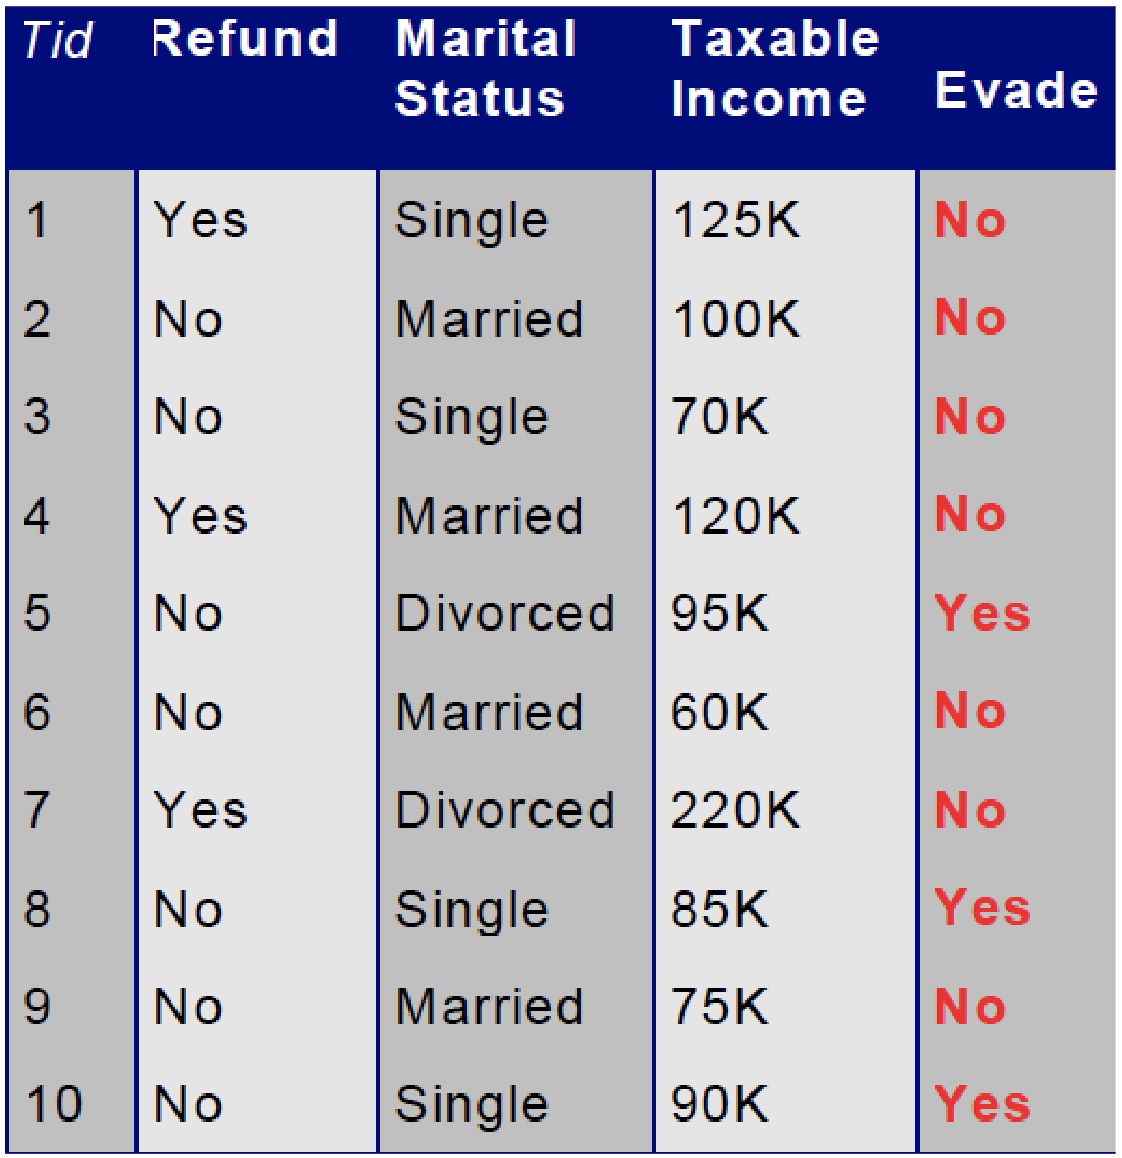
\includegraphics[width=0.5\linewidth]{img/NBC.png} 
\end{figure}

Then, $P(Evade = Yes) = 3/10$, and $P(Marital_Status = Single | Evade = Yes) = 2/3$.

Datasets, however, often contain continuous data. In order to deal with such attributes, the solutions can be:
\begin{itemize}
    \item Discretization of the values into bins, although it would violate the independence assumption;
    \item Two way split, so the values are split into two intervals and we choose one of them;
    \item We use a \textbf{probability density distribution}. This means that we assume a certain distribution function for the variable and use it on unseen data.
\end{itemize}

A commonly used distribution function is the \textbf{Gaussian/normal distribution function}:

\begin{equation*}
    P(X_i = x_i | Y = yi) = \dfrac{1}{\sqrt{2 \pi} \sigma_{ij}} e^{-\frac{(x_{ij} - \mu_{ij})^2}{2 \sigma_{ij}^2}} \, ,
\end{equation*}
where the mean $\mu_{ij}$ can be estimated as the mean of $X_i$ for all the records belonging to class $y$, and the variance $\sigma_{ij}^2$ can be estimated as the sample variance $s^2$ of the same records.

One thing to notice is that if the conditional probability for any attribute is 0, then the likelihood will be 0 as well. Zero conditional probabilities arise then the number of training instances is small and the number of possible values of an attribute is large. The Naïve Bayes Classifier, as is, cannot classify records when this happens. To address the problem, it is important to adjust the conditional probability estimates so that they are not simple fractions of training instances. This can be achieved by using the following alternate estimates of conditional probability:

\begin{equation*}
    P(X = x| Y = y) = \dfrac{N_{xy} + 1}{N_y + v} \, \text{(\textbf{Laplace estimate})},
\end{equation*}

\begin{equation*}
    P(X = x| Y = y) = \dfrac{N_{xy} + mp}{N_y + m} \, \text{(\textbf{M-estimate}}.
\end{equation*}
Here, $v$ is the total number of attribute values that $X$ can take. $p$ is an initial estimate of $P(X = x | y)$ that is known a priori, and $m$ is an hyperparameter that represents our confidence in using $p$ when the fraction of training examples is too brittle. Note that these estimates provide non-zero values even when $n_c = 0$.

Summing up, Naïve Bayes Classifiers:
\begin{itemize}
    \item are robust to isolated noise points since they don't significantly influence the conditional probability estimates;
    \item can easily compute probabilities even in high-dimensional spaces, provided attributes are actually conditionally independent of each other giver the class labels;
    \item can handle missing values in both training and test instances, by simply ignoring them.
    \item are robust to irrelevant attributes, because if $X$ is an irrelevant attribute, then $P(X=x|Y=y)$ becomes almost uniformly distributed.
\end{itemize}
In case the Naïve Bayes Assumption does not hold, we need to use different frameworks, such as Bayesian Networks.

\section{Decision Tree Classifier}

To illustrate how a decision tree works, we will use a practical example. Imagine a classification problem in which the data is represented by vertebrate animals, and the target is to distinguish them into mammals and non-mammals. One approach to solve the classification problem is to pose a series of questions about the characteristics of the animal. Is it cold-blooded? If yes, it's a reptile. Otherwise, does it have feathers? Again, if yes, it's a bird. So, if it's warm-blooded and has no feathers, it's a mammal.

In general, we can ask a series of questions about the attributes of the instance, and for each answer we receive, we can either give a verdict or ask a new question, until the instance is classified. The questions and answers can be organized in a \textbf{decision tree}. A decision tree has three types of nodes:
\begin{itemize}
    \item A \textbf{root node}, with no incoming links and $l \in \mathbb{N}$ outgoing links;
    \item \textbf{Internal nodes}, each with one incoming link and $l \in \mathbb{N} \setminus \{0,1\}$ outgoing links;
    \item \textbf{Leaf/terminal nodes}, each with one incoming link and 0 outgoing links.
\end{itemize}
Every leaf is associated with a class label, while the internal nodes are associated to an attribute test condition, typically defined using only one attribute at a time. Each possible outcome is associated with a child of the node.

Given a decision tree, classifying an unseen instance is straightforward: starting from the root, choose the child that corresponds to the answer of the attribute test, and stop once a leaf node is reached. The outcome in the leaf node will be the output of the model on that instance. By constructing a decision tree for the previous animal example, if we were to classify the following instance:
\begin{table}[h!]
    \centering
    \begin{tabular}{c|c|c}
        name & coldBlood & feathers \\
        \hline
        owl & no & yes \\
    \end{tabular}
\end{table}

we would answer "no" and "yes" to the first two questions, thus classifying it as a non-mammal. But how is the decision tree built?

\subsection{Decision Tree Induction}

There's a few different algorithms that can build decision trees. One of the earliest ones is \textbf{Hunt's algorithm}, which is also the basis for more recent ones such as \textbf{ID3}, \textbf{C4.5}, and \textbf{CART}.

\subsubsection{Hunt's algorithm}

In this algorithm, the decision tree is built recursively. The tree initially contains only one node, the root, associated with all the training instances. If it's associated with instances belonging to multiple classes, it is expanded using an attribute test condition determined through a \textbf{splitting criterion}. A child leaf node is constructed for all possible outcomes of the test, and the instances of the father are distributed among them. This expansion is repeated recursively on all leaves, until a leaf can no longer be expanded since it represents only one class label.

This algorithm makes some simplifying assumptions that are often not true in practice:
\begin{itemize}
    \item Some of the child nodes may be empty if none of the training examples have the particular attribute values; one way to handle this is to declare each of them as a leaf node with a class label that occurs most frequently among the training instances associated with the parent node.

    \item If all training instances associated with a node have identical values, it's not possible to expand the node. One way to handle the problem is to declare the node as a leaf and assign it to the class label that occurs most frequently in it.
\end{itemize}

\subsubsection{ID3, C4.5, CART}

ID3 uses Hunt's algorithm with information gain criterion and gain ratio. C4.5 improves ID3, but needs all the data to fit in memory, can handle missing values for continuous attributes, performs tree post-pruning, and is unsuitable for large datasets. CART builds multivariate decision binary trees.

\subsection{Design Issues In Tree Induction}

Hunt's algorithm is a generic procedure for growing decision trees in a greedy fashion. To implement the algorithm, there are two key design issues to address:

\begin{itemize}
    \item \textbf{The splitting criterion}, so which attribute to select at each iteration to partition the dataset, and how should the instances be distributed to child nodes.

    \item \textbf{The stopping criterion}, so when expanding of nodes should stop. Obviously, if we run the algorithm with no restrictions, it will eventually only find unsplittable leaf nodes and terminates. However, we may still choose to interrupt the splitting on nodes even if they contain instances of more than one class to avoid overfitting of the training data, using a regularization technique called \textbf{early termination/early stopping}.
\end{itemize}

\subsection{Methods for Expressing Attribute Test Conditions}

Induction algorithms must provide a method for expressing an attribute test condition and corresponding outcomes for different attribute types.

For \textbf{binary attributes}, the test condition will generate two possible outcomes. For \textbf{nominal attributes}, which may have multiple values, the attribute test condition can be expressed either as a binary split, isolating one or more value from all the rest, or a multiway split, with one new node for each value. For \textbf{ordinal attributes}, the attribute test condition can also produce either a binary or multiway split, but the grouping in the binary one must respect the order property of the values. For \textbf{continuous attributes}, the attribute test condition can be expressed as a comparison test producing a binary split, or a range query through discretization producing a multiway split. In this last case, discretization may be static (the values are discretized once at the beginning), or dynamic (the discretization is repeated at each node).

\subsection{Methods for Selecting an Attribute Test Condition}

There are many measures that can be used to determine the goodness of an attribute test condition. These measures try to give preference to attribute test conditions that partition the instances into purer subsets in the child nodes, which means that each child contains instances belonging mostly to one class. Having a purer subset means that the corresponding node will be expanded less (or not at all, if it contains only one class), while having impure subsets may require a lot of splits and therefore a deeper tree, which might be susceptible to overfitting.

The idea is to calculate the \textbf{impurity} of a node through an appropriate measure, both before and after splitting, and to choose the attribute test condition that produces the highest $Gain = Impurity_{pre} - Impurity_{post}$ (or, equivalently, the lowest impurity measure after splitting). The following are some commonly used impurity measures; $p_i(t)$ refers to the relative frequency of training instances that belong to class $i$ at node $t$, and $c$ is the total number of classes.

\BoxDef{Gini Index}{
\begin{equation*}
   Gini = 1 - \sum_{i=0}^{c-1} p_i(t)^2
\end{equation*}
Maximum: $1-1/c$ \hfill Minimum: $0.0$
}
The Gini Index for a collection of nodes is calculated as:
\begin{equation*}
    Gini_{split} = \sum_{i=1}^k \dfrac{n_i}{n} Gini(i) \,,
\end{equation*}
where $n_i$ is the number of records at child $i$ and $n$ is the number of records at parent node $p$. To choose the attribute for the current split to perform, we select the one that minimizes the weighted average Gini index of the children.

For categorical attributes, the count matrix is calculated considering each distinct value, and an index is produced for the different possible multiway/binary splits.

For continuous attributes, the construction of the count matrix is not as immediate. The split is done by choosing one or more threshold values to separate instances based on a inequality test: for a basic binary split, a value $v$ must be chosen so that one child node will contain all instances with $attr \leq v$, and the other child node will contain all instances with $attr > v$. The bruteforce approach to find the idea value of $v$ is to pick one value of the attribute at a time to use as a threshold, scan the database to compute the count matrix, and determine the Gini index. This approach is obviously inefficient, with a complexity of $O(n^2)$ (where $n$ is the number of training instances).

A more efficient algorithm is the following:
\begin{enumerate}
    \item the instances are sorted by value of the attribute;

    \item the split positions are calculated as the midpoints between every couple of adjacent sorted values;

    \item the new splits are linearly scanned updating each time the count matrix and Gini index;

    \item the split position is chosen as the one with the lowest index.
\end{enumerate}
This algorithm has a complexity of $O(nlog(n))$.

\BoxDef{Entropy}{
\begin{equation*}
    Entropy = - \sum_{i=0}^{c-1} p_i(t) \log_2 (p_i(t))
\end{equation*}
Maximum: $\log_2(c)$ \hfill Minimum: $0.0$
}

The entropy is used the same way as the Gini index: the lower the value, the better the split.

\BoxDef{Classification Error}{
\begin{equation*}
    Classification \; error = 1 - \max_i p_i(t)
\end{equation*}
Maximum: $1-1/c$ \hfill Minimum: $0.0$
}

Overall, all three measures are coherent with each other, but may lead to different choices in terms of what attributes to use for the split. 

\subsubsection{Gain Ratio}

One limitation of impurity measures is that the tend to favor qualitative attributes with large number of distinct values. Having a low impurity value alone is not enough to find a good attribute test condition for a node. There are two ways to overcome this problem: one way is to generate only binary decision trees, avoiding the problem of handling attributes with varying values altogether. Another way is to modify the splitting criterion to consider the number of partitions produced by the attribute as well.

In the C4.5 algorithm, a measure known as \textbf{gain ratio} is used, which compensates for attributes that produce a large number of child nodes.

\BoxDef{Gain ratio}{
The gain ratio is calculated as:
\begin{equation*}
    Gain \; ratio = \dfrac{Gain}{Split \; info} = \dfrac{Entropy(p) - \sum_{i=1}^k \dfrac{N(v_i)}{N} Entropy(v_i)}{- \sum_{i=1}^k \dfrac{N(v_i)}{N} \log_2(\dfrac{N(v_i)}{N})}
\end{equation*}
where $N(v_i)$ is the number of instances assigned to node $v_i$, and $k$ is the total number of splits.
}

\subsection{Algorithm for Decision Tree Induction}

We can now present a full pseudocode for a decision tree induction algorithm.

\begin{algorithm}
\caption{Pseudocode for a decision tree induction algorithm.}
\texttt{TreeGrowth}$(E,F)$
\begin{algorithmic}[1]
        \If{\texttt{stopping\_cond}$(E,F)$}
            \State leaf = \texttt{create\_node()}
            \State leaf.label = \texttt{classify}$(E)$
            \State return leaf
        \Else
            \State root = \texttt{create\_node()}
            \State root.testcond = \texttt{find\_best\_split}$(E,F)$

            \For{$v \in $ root.testcond.outcome}
                \State $E_v$ = $\{e | root.testcond(e) = v and e \in E \}$
                \State child = \texttt{TreeGrowth}$(E_v,F)$
                \State add child as descendant to root and label the edge as $v$.
            \EndFor
        \EndIf
        \State return root.
\end{algorithmic}
\end{algorithm}

\subsection{Advantages of Decision Tree Classifiers}

The following is a summary of the most important characteristics of decision trees and decision tree induction algorithms.

\paragraph{Applicability}
Decision trees are a non-parametric approach to build a classification model. It does not require any prior knowledge about the probability distribution of the values, nor any type of normalization.

\paragraph{Easy to interpret}
If the tree is small enough, it's also going to be easy to read.

\paragraph{Expressiveness}
A decision tree can encode any discrete-valued function, since they can be represented by an assignment table where each combination of attribute values is associated with a class label. It does not generalize well to certain types of Boolean functions (e.g., parity function). It also greatly struggles with continuous variables, especially when test conditions involve only a single attribute at a time.

\paragraph{Computational efficiency}
Decision tree induction algorithms typically employ an heuristic-based search in the hypothesis space. These searches can construct a reasonably good decision tree quickly even with large datasets (with a complexity of $O(m nlog(n))$, where $m$ is the number of attributes and $n$ is the number of instances). Also, once a decision tree has been built, the cost of classifying a new instance is $O(w)$, where $w$ is the maximum depth of the tree.

\paragraph{Handling of missing values}: missing values can be dealt with in different ways, both in the training set and in the test set. If there's missing values in the test set, the classifier must choose which path to follow if a value is missing for a given test instance. The \textbf{probabilistic split method} (used by the C4.5 classifier) distributes the data instance to every child of that node according to the probability that the missing attribute has a particular value. In another approach, known as \textbf{surrogate split method} (used by the CART classifier), the instance whose splitting attribute value is missing is assigned to one of the child nodes based on the value of another non-missing surrogate attribute whose splits most resemble the partitions made by the missing attribute. The \textbf{separate class method} (used by the CHAID algorithm) treats the missing value as a separate categorical value. Alternatively, data preprocessing is needed to replace missing values with a mean or a mode.

During training, if an attribute $v$ has missing values in some training instances associated with a node, we need to measure the gain of purity if $v$ is used for splitting. One way to do so it to just exclude instances with missing values of $v$ in the counting instances associated with every child node. If $v$ is chosen, then the instances with missing values can be propagated to children using the methods seen for testing.

\paragraph{Handling of irrelevant and redundant attributes}
An attribute is irrelevant if it is not useful for the task, while it is redundant if it is strongly correlated with some other attribute in the data.
    
Since irrelevant attributes are poorly associated with the target class labels, they will provide little to no gain in purity and will not be chosen for attribute test conditions. However, not all attributes that bring poor gain in purity are also irrelevant, so in more complex classification problems, irrelevant attributes may still be favored over more relevant ones with poorer gain. Feature selection techniques can help to improve the accuracy of decision trees by eliminating them.

As for redundant attributes, since they will show similar gains to the ones they're correlated with, only one of them will be chosen for the attribute test condition for a node.

\paragraph{Robustness w.r.t noise}
*?

\paragraph{Poor handling interactions among attributes}
Attributes are considered interacting if they are able to distinguish between classes when used together, but individually they don't provide any information. Due to the greedy nature of the splitting criterion, these attributes may be ignored in favor of other attributes that are actually not as useful, thus producing a tree more complex than needed.

\paragraph{Space of tree possibly exponentially large}
Since we use a greedy approach, we often cannot find the optimal tree.

\paragraph{Rectilinear decision boundaries}
Since each split is done considering one attribute at a time, the decision boundary is going to be rectilinear, i.e., composed of lines parallel to the axes. A more accurate approximation of the real decision boundary can be obtained with \textbf{oblique decision trees}, which allow multiple attributes to be tested at each node. Although they can produce more compact trees and are more expressive, they are also more computationally expensive to construct, since finding the optimal test condition is not as easy.

\paragraph{Data fragmentation}:
As the tree is traversed, the number of instances gradually gets smaller. The number of instances in the leaves could potentially be too small to make any statistically significant decision.

\paragraph{Tree replication}
The final tree may need to have some replicated subtrees (think of the one constructed to approximate the boolean parity function). The need for replication means that it takes longer to learn the tree, and replicated subtrees learned further down must be learned using a smaller training subset. Some approaches to deal with replication include constructing a \textbf{decision graph}, where children may have more than one parent, or using obliue decision trees with multivariate tests at each node.

\section{Model Evaluation}
\subsection{Metrics for Model Evaluation}

The most basic approach for representing a classifier's performance on a test set is to use a \textbf{confusion matrix}. A confusion matrix summarizes the number of instances predicted correctly or incorrectly by the model, using the following counts:

\begin{itemize}
    \item \textbf{True Positive (TP)}, or $f_{++}$, which corresponds to the number of positive examples correctly classified;

    \item \textbf{False Positive (FP)}, or $f_{-+}$, which corresponds to the number of positive examples incorrectly classified as negative;

    \item \textbf{True Negative (TN)}, or $f_{--}$, which corresponds to the number of negative examples correctly classified;

    \item \textbf{False Negative (FN)}, or $f_{+-}$, which corresponds to the number of negative examples incorrectly classified as positive.
\end{itemize}

The confusion matrix is drawn as follows:

\begin{table}[h]
    \centering
    \begin{tabular}{|c|c|c|}
         \hline
         & pred. + & pred. - \\
        \hline
        actual + & $f_{++}$ & $f_{-+}$\\
        \hline
        actual - & $f_{+-}$ & $f_{--}$\\
        \hline
    \end{tabular}
\end{table}

These counts are summarized using a number of \textbf{evaluation measures}.
All these measures can be generalized by the \textbf{weighted accuracy}, calculated as:
\begin{equation*}
    WAccuracy = \dfrac{w_1a + w_4d}{w_1a + w_2b + w_3c + w_4d} \, .
\end{equation*}

\bgroup
\def\arraystretch{1.5}%
\begin{table}[ht]
\scriptsize
    \centering
    \begin{tabular}{ 
    | >{\centering\arraybackslash}p{90pt}
    | >{\centering\arraybackslash}p{140pt}
    | >{\centering\arraybackslash}m{100pt} | }
    
    \hline
        True positive rate (Sensitivity, Recall) & $TPR = \dfrac{TP}{TP + FN}$ & Measures the rate at which positive instances are correctly classified. \\
        \hline
        True negative rate (Specificity) & $TNR = \dfrac{TN}{TN + FP}$ & Measures the rate at which negative instances are correctly classified. \\
        \hline
        False positive rate (False alarm) & $FPR = 1 - TNR$ & Measures the rate at which positive instances are incorrectly classified. \\
        \hline
        False negative rate & $1 - TPR$ & Measures the rate at which negative instances are incorrectly classified. \\
        \hline
        Accuracy & $ Accuracy = \dfrac{TN + TP}{TN + TP + FN + FP}$ &  Measures the rate of correctly classified instances. \\
        \hline
        Precision (positive predicted value) & $Precision = \dfrac{TP}{TP + FP}$ & Measures how likely is the classifier to have most of its positive predictions be correct. \\
        \hline
        False discovery rate & $FDR = 1 - Precision$ & Measures how likely is the classifier to have most of its positive predictions be incorrect. \\
        \hline
        F-Measure & $F = \dfrac{2rp}{r+p} = \dfrac{2TP}{2TP + FN + FP}$ & Measures how likely is the classifier to have most of its positive predictions be incorrect. \\
    \hline
    \end{tabular}
\end{table}
\egroup

\clearpage

The most widely used is accuracy, although it's not suitable when classes are not balanced, since it tends to favor classifiers that correctly classify the majority class.

A \textbf{cost matrix} can be defined to assign specific costs to different counts:
\begin{table}[h]
    \centering
    \begin{tabular}{|c|c|c|}
         \hline
        $C(i|j)$ & pred. + & pred. - \\
        \hline
        actual + & $C(+|+)$ & $C(-|+)$\\
        \hline
        actual - & $C(+|-)$ & $C(-|-)$\\
        \hline
    \end{tabular}
\end{table}
Each $C(i|j)$ is the cost of misclassifying class $j$ as class $i$. The cost of classification is calculated the same as accuracy, except each term is multiplied by the corresponding cost.

Accuracy is proportional to cost if $TP = TN = p$ and $FP = FN = q$; accuracy would be calculated as $(TP + TN)/tot$, and the cost as:

\begin{align*}
    Cost = p(TP + TN) + q(FP + FN) \\
    = p(TP + TN) + q(tot - TP - TN) \\
    = qtot - (q - p)(TP + TN) \\
    = tot(q - (q-p)Accuracy).
\end{align*}

If we have a multiclass classifier, then we calculate each measure for a single class at a time against all others. So, for example, if we have 3 classes A, B, and C, a false positive for A happens if the classifier identifies an element of either B or C as belonging to A.

\subsection{Methods for Performance Evaluation}

The three main steps needed to construct a model are training to adjust the parameters, validation to choose the best hyperparameters, and testing to estimate the "goodness" of the final model. It's of fundamental importance that the model is not tested on data it already saw during training, because that would produce inaccurately optimistic evaluations. Once the estimation has been done, if it's sufficiently good the model can be accepted and retrained on all the data (since the more data is used to train the model, the better its generalization capabilities will be). If the estimate is bad, it must be discarded and rebuilt with different parameters/hyperparameters; we cannot go back to validation and adjust only the hyperparameters, as that would be a choice made looking at the test set.

How can we obtain a reliable estimate of performance? Consider that performance depends on many factors, such as class distribution in the dataset, cost of misclassification, and the size of the training and test sets.

First of all, we need to find the smallest number of data records the model needs to produce an accurate estimate on new inputs. This can be done by drawing the learning curve, obtained by plotting the amount of data used against the accuracy. Typically, accuracy is evaluated by training on datasets of sizes increasing in powers of 10. The minimum size of the dataset can be chosen as the x value after which accuracy does not improve significantly.

\begin{figure}[h]
    \centering
    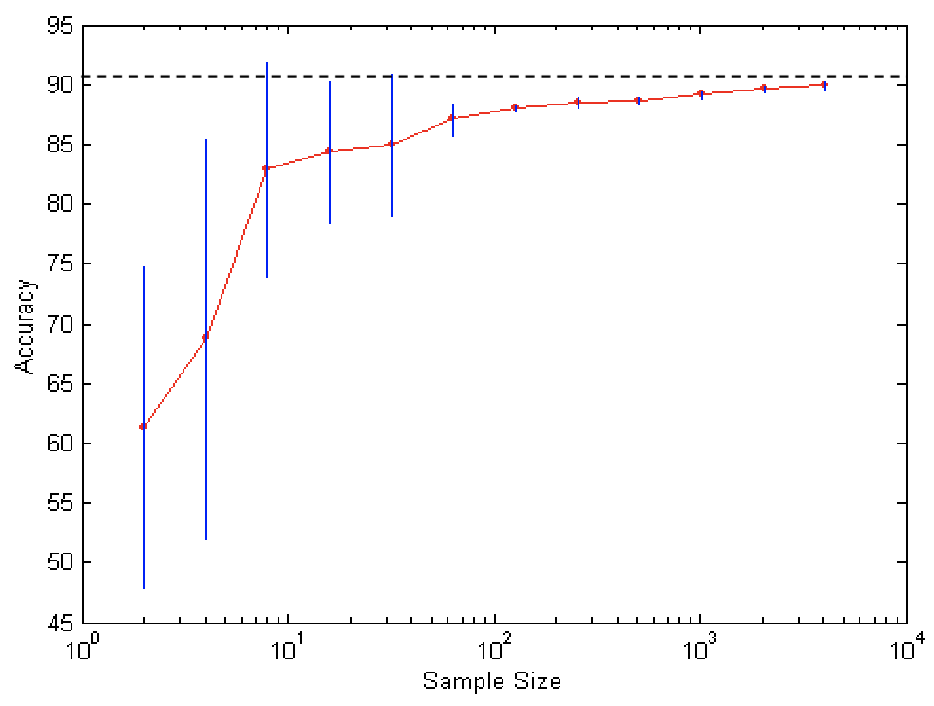
\includegraphics[width=0.5\linewidth]{img/Learning curve.png}
    \caption{The learning curve plotted for different sizes of the training dataset.}
\end{figure}
In the figure above, we may choose $10^2$ as the ideal size of the dataset. This method needs caution, since s sample size too small may show bias in the data represented or too much variance in the estimate.

There are many techniques for model assessment and evaluation, such as holdout, random subsampling (randomized repeated holdout), cross validation, stratified sampling, bootstrap, etc. (SEE ML NOTES).

\textbf{Holdout} is simple, but uses only part of the data for training and part for testing. Repeated holdout performs holdout multiple times by choosing the test set randomly each time, and the final estimation is the mean across all evaluations. This approach is still not optimal, since the test set of one iteration may overlap with the test set of another.

A better technique is \textbf{K-fold cross validation}. The dataset is partitioned into $K$ parts; then, for each value of $K$, the $K^{th}$ part is taken as the validation/test set, while the rest is the training/training + validation set. Often, it is used in conjunction with stratification to make sure that each part represents the target classes equally. After performing the validation/testing on all $K$ parts, the error is calculated as the average across all folds. This provides a better estimate than simple holdout methods.

\subsection{Methods for Model Comparison}

\subsubsection{ROC Curve}

Assessing the performance of a classifier over a range of score thresholds is called \textbf{aggregate evaluation} of performance. One of the widely used tools for aggregate evaluation is the \textbf{Receiver Operating Characteristic (ROC) curve}. A ROC curve is a graphical approach to visualize the trade off between TPR (true positive rate, plotted in the y axis) and FPR (false positive rate, plotted on the x axis) of a classifier. It shows he ability of a binary classifier as the discrimination threshold is varied, so each point corresponds to a different threshold value.

The following procedure describes the generic approach for computing a ROC curve:

\begin{enumerate}
    \item Sort the test instances in increasing order of their scores (can be posterior probability calculated using some other classifier).

    \item Select the lowest ranked test instance (with the lowest score), and assign that instance and all the ones ranked higher to the positive class. Since all the positive instances are classified correctly and all negative one are misclassified, $TPR = FPR = 1$.

    \item Select the next test instance from the list. Classify the selected instance and those ranked higher as positive, anything below as negative. Update TP and FP counts accordingly.

    \item Repeat the previous step and update TP and FP counts until the highest ranked instance is selected. At this final stage, $TPR = FPR = 0$.

    \item Plot the TPR against the FPR.
\end{enumerate}

A perfect model with 0 misclassifications would have $FPR = 0$ and $TPR = 1$. To summarize the aggregate behaviour across all operating points, one of the most commonly used measures is the \textbf{area under the ROC curve (AUC)}. If the classifier is perfect, the AUC is equal to 1. If the classifier is bad, and behaves as a random guesser, the AUC will be 0.5.

Note that when comparing different models using AUC, we cannot say that a model is better than another for simply having an higher AUC (unless the difference is drastic enough). Consider the ROC curves for the models $M_1$ and $M_2$ pictured below:

\begin{figure}[h]
    \centering
    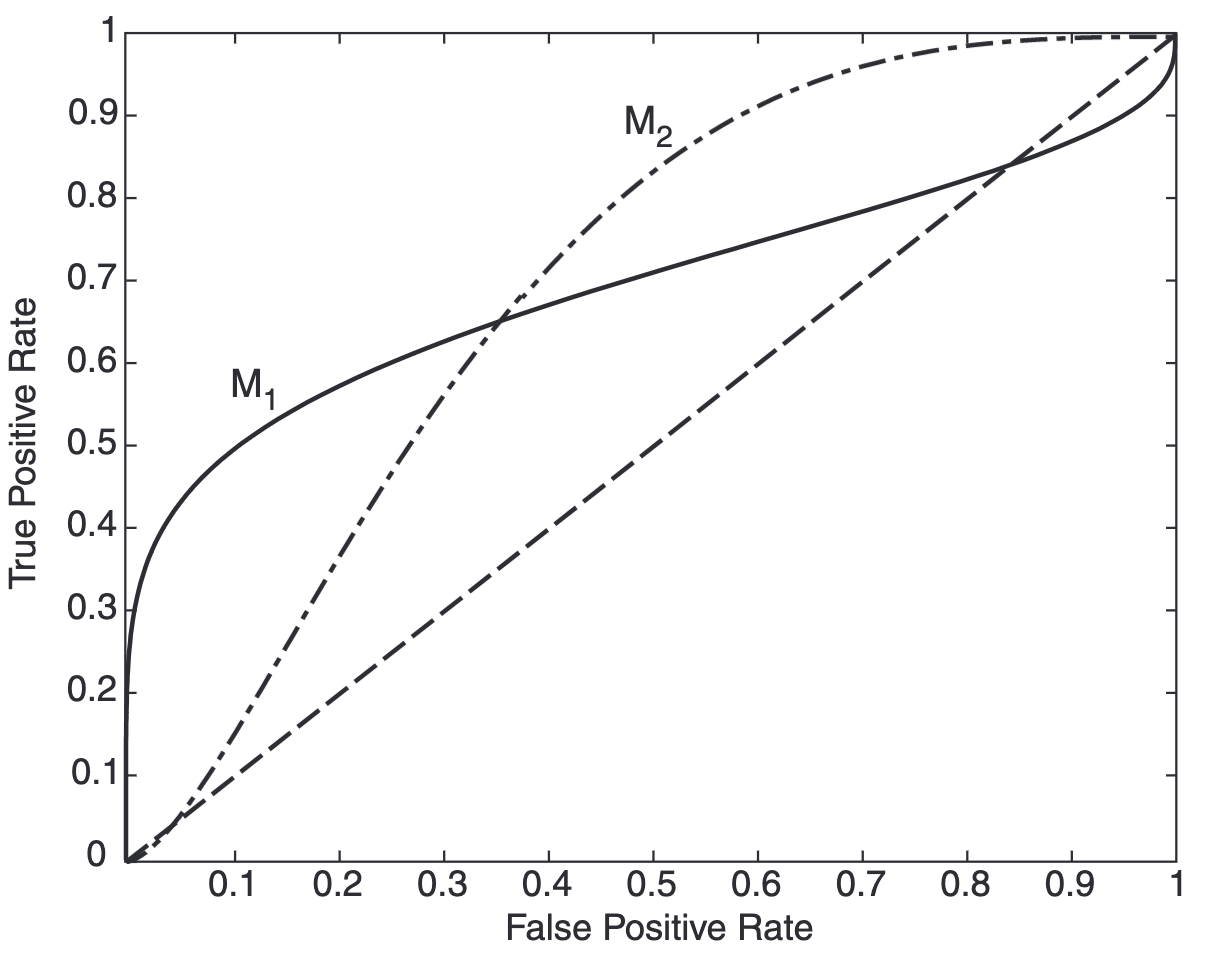
\includegraphics[width=0.5\linewidth]{img/ROC_comparison.png}
    \caption{ROC curves for two different classifiers.}
\end{figure}

$M_2$ does have a slightly bigger AUC compared to $M_1$, but they are both good at different things: $M_1$ is better for small FPR, while $M_2$ is better for large FPR.

\subsubsection{Lift Chart}

The \textbf{lift chart} (or \textbf{gains chart}) is another popular technique, used often in direct marketing. The input is a dataset where each ``case'' is scored with the estimated probability that it will belong to a given class. The lift chart is the constructed by plotting the cumulative number of cases (on the x axis) against the cumulative number of true positives (on the y-axis). 

\begin{figure}[h]
    \centering
    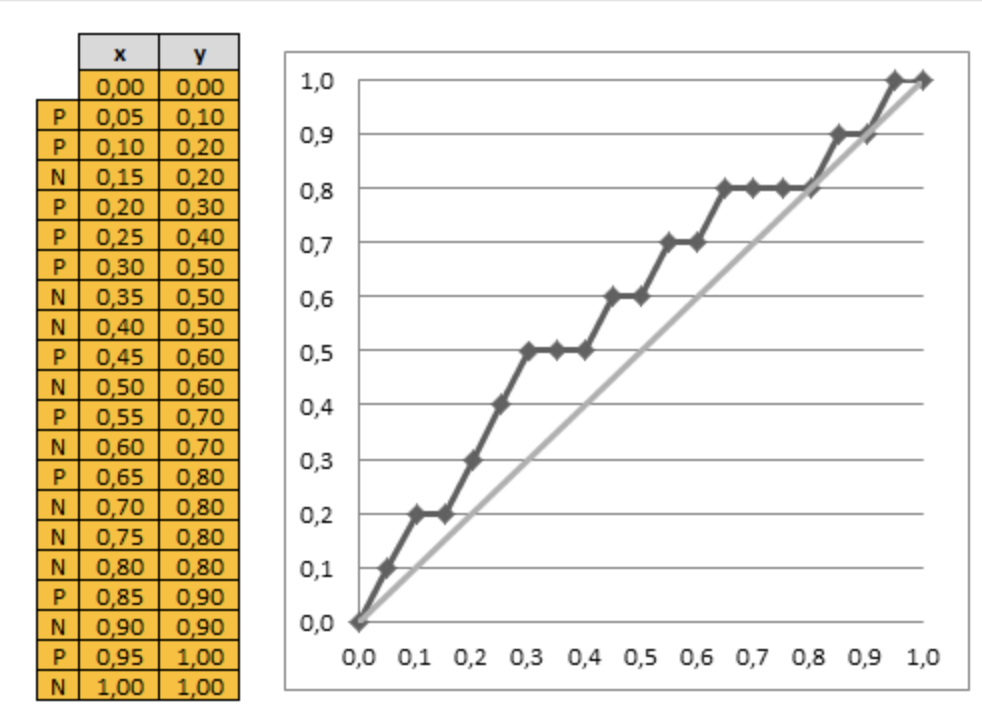
\includegraphics[width=0.5\linewidth]{img/Lift chart.png}
    \caption{Example of lift chart.}
\end{figure}

The gray line is a reference line. For any given number of cases, it represents the expected number of positives we would predict if we did not have a model, but simply selected at random (similarly to the line in the middle of the ROC curve plot).

From this chart, we can derive an economical value plot; e.g., given a predictive model for target marketing, how many customers should we target to maximize income? The profit is given by the following formula: $UnitB * MaxR * Lift(X) - UnitCost*N*X/100$, where $UnitB$ is the unit benefit, $MaxR$ is the expected number of potential responders in the population considered (of size $N$), $Lift(X)$ is the lift chart value for $X \in [0,1]$, and $UnitCost$ is the unit postal cost.

\begin{figure}
    \centering
    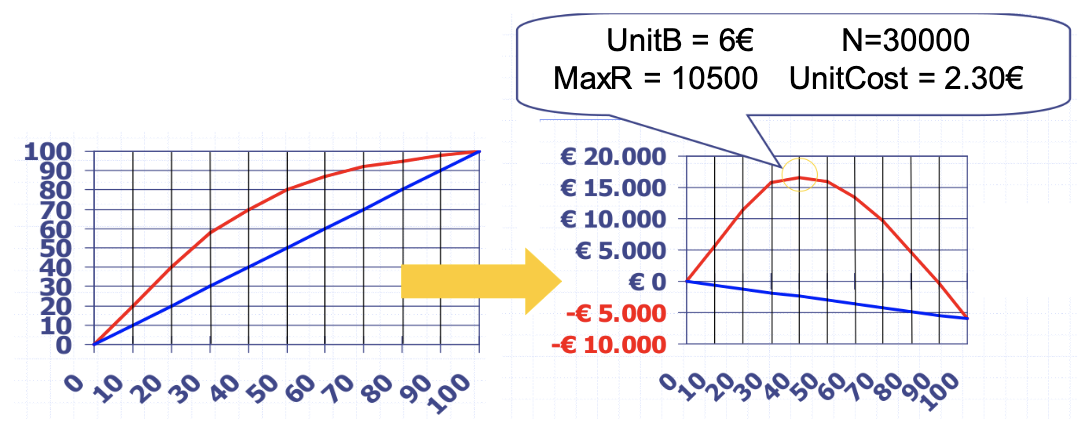
\includegraphics[width=0.5\linewidth]{img/Lift chart application.png}
    \caption{Example of application of a lift chart.}
\end{figure}


\section{Issues of Classification}

\subsection{Underfitting and Overfitting}

As of now, we considered algorithms that construct models with the lowest possible training error. In practice, however, if a model fits the data too much, it incurs into \textbf{overfitting}. Overfitting happens when the training error is very low, but the generalization error is high. This means that the model is too adapted to the training data (also said to be ``overtrained''), and cannot accurately predict unseen instances. \textbf{Underfitting} is the opposite phenomenon, when the model is not adapted enough to the training data, thus producing an also high generalization error. These phenomenons are controlled by the \textbf{complexity} of the model. Each model has a different way to measure this complexity. In the case of a K-NN classifier, the complexity is inversely proportional to the number of neighbors that make a neighborhood. For decision trees, the complexity is proportional to the depth of the tree.

Another problem that can cause overfitting regardless of the training/validation procedure is the lack of sufficient training examples. The likelihood of incurring into overfitting is inversely proportional to the number of the available training instances. 

\textbf{The course slides seem to imply that overfitting can be caused by the mere presence of noisy data. This is inexact; overfitting is caused by having a model so complex it adapts too much to noisy data, but the presence itself of noise should not be a concern given appropriate regularization.}

\subsection{Model Selection}

Model selection is the phase in which the model's parameters and hyperparameters are chosen. This is done by using a training set along with a \textbf{validation} set (containing instances selected from the training set). The model is first set up with some starting values of parameters and hyperparameters. The model is trained on the training set, and the generalization error is estimated by the error calculated on the validation set. After a model with an acceptable validation error is selected, its quality is assessed using the test set instances.

There's many ways to divide the data to perform training, validation, and testing. The simplest way is \textbf{hold-out}, in which the training set is split into three partitions, one for testing, one for validation, and one for testing. This technique, however, ``wastes'' the data as only some of it can be used for each step. Another technique is \textbf{k-fold cross validation} (it can be used for testing as well, either in combination with hold-out, or with cross-validation). The dataset $D$ is split into $k$ partitions; then, for each partition $D_i$, training is done using $D / D_i$, and validation is performed using $D_i$ only. This way, testing and validation is repeated multiple times with different data, obtaining a more accurate estimation of the generalization error.

To select the final model, the strategy used is inspired by \textbf{Occam's razor/principle of parsimony}: when presented with two models with the same errors, the simpler model is preferred over the more complex one; again, we prefer simpler models because they're less likely to fall into overfitting. One way to estimate the generalization error of the model is:

\begin{equation*}
    R(Model) = R_{emp}(Model, TR) + \alpha Complexity(Model)
\end{equation*}

\subsection{Model Assessment}

There's three ways to estimate the generalization error:
\begin{itemize}
    \item \textbf{Pessimistic estimate}: the generalization error rate is assumed to be worse than the training error rate;
    \item \textbf{Optimistic/resubstitution estimate}: the generalization error rate is assumed to be the same as the training error rate;
    \item \textbf{Reduced error pruning (REP)}: the generalization error rate is assumed to be the same as the validation error rate.
\end{itemize}

Let's consider error estimation for decision tree classifiers. The pessimistic error estimate for a decision tree $T$ with $k$ leaf nodes is:

\begin{equation*}
    R(T) = R_{emp}(T) + \omega \dfrac{k}{N_{train}} \,,
\end{equation*}
where $\omega$ is the cost of adding a leaf node, and $N_{train}$ is the number of training instances.

The optimistic error estimation would simply be:
\begin{equation*}
    R(T) = R_{emp}(T)
\end{equation*}

\subsection{Addressing Overfitting in Decision Trees}

A common regularization technique used for decision trees is \textbf{pre-pruning}, which is a form of early stopping. The training algorithm is stopped before the tree is fully formed, without necessarily having all leaf nodes with instances of one class only. We can set new conditions such as:
\begin{itemize}
    \item the number of instances is less than some user-defined threshold;
    \item the class distribution of instances is independent from the available features (e.g. tested using a $\chi^2$ test);
    \item the current node does not improve impurity measures;
    \item the estimated generalization error falls below a certain acceptable threshold.
\end{itemize}

Alternatively, we can employ \textbf{post-pruning}. The decision tree is grown in its entirety; then, nodes are trimmed from the bottom. If a trimming improves the generalization error, it's accepted, replacing the pruned subtree with a single leaf. The label corresponding to the leaf is chosen as the majority class of instances in the subtree.

\chapter{Regression}

Another common supervised learning task is regression. While classification assigns to each instance a class (out of a finite set of classes), regression predicts a real-valued number. More formally: given a training set $<x_i, y_i>$ for some unknown target function $f$, regression is the task of learning $f$ by finding a good approximation; that is, one that minimizes the error. The error function can be expressed in many ways; some common functions are \textbf{absolute error}:
\begin{equation*}
    \sum_i |y_i - f(x_i)| \,,
\end{equation*}
and \textbf{squared error}:
\begin{equation*}
    \sum_i (y_i - f(x_i))^2 \,,
\end{equation*}
where $(y_i - f(x_i))$ is called \textbf{residual}.

\section{Linear Regression}

Linear regression models a linear relationship between a dependent variable $Y$ and a set of one or more independent variables $X$. The target function is expressed as a linear function:
\begin{equation*}
    f(x) = \sum_i^n a_i*x_i + b = a^T*x + b\,,
\end{equation*}
where $b$ is called \textbf{intercept} (or \textbf{bias}) and the vector $a$ is the \textbf{slope}. These are called free parameters. If we consider only one independent variable, the task is called \textbf{simple linear regression}, otherwise it's called \textbf{multiple linear regression}. For multiple correlated dependent variables, the task is called \textbf{multivariate linear regression}.

The goal is to find some hypothesis (approximation of the target function $f$) that for each input instance returns the expected value for that input according to $f$. This approximation corresponds to the function $h$ that minimizes the error for each $x_i$ in the training set, i.e., it minimizes the residual $(y_i - h(x_i))$.

There's many ways to find the values of $a$ and $b$ such that $h(x) = \sum_i a_i * x_i + b$ minimizes the error; one of the most common approaches is \textbf{gradient descent}. Since the error function is a simple convex function, it will certainly have a global minimum. By differentiating the error function in all $a_i$ and $b$ and setting it to 0, we can find the exact values of the free parameters that correspond to the minimum. Let's use the Least Squares method to minimize the error, calculated as the SSE, also known as \textbf{residual sum of squares}. The free parameters will be referred to as the weight vector $w$ from now on, to simplify notation:
\begin{equation*}
    E(w) = \sum_i^n (y_i - w^T*x_i))^2 
\end{equation*}
(here $b$ is incorporated into $w$ as $w_0$, and $x_0$ is assumed to be 1). The gradient of the error function for a generic $w_j$ is calculated as follows:
\begin{gather*}
    \dfrac{\partial E(w)}{\partial w_j} = \dfrac{\partial \sum_i^n (y_i - w^T*x_i))^2}{\partial w_j} = 2 \sum_i^n (y_i - w^T*x_i) \dfrac{\partial \sum_i^n (y_i - w^T*x_i))}{\partial w_j} = \\
    2 \sum_i^n (y_i - w^T*x_i) (\dfrac{\partial \sum_i^n y_i}{\partial w_j} +\dfrac{\partial \sum_i^n w^T x_i}{\partial w_j}) = 2 \sum_i^n (y_i - w^T*x_i) ( 0 + \sum_i^n x_{i,j}) = \\
    2 \sum_i^n (y_i - w^T*x_i) x_{i,j} \,,
\end{gather*}
where $x_{i,j}$ refers to the $j^{th}$ attribute of the $i^{th}$ example. By setting this to 0 for all $w_i$, we find that:
\begin{gather*}
    \dfrac{\partial E(w)}{\partial w_0} = \dfrac{\partial E(w)}{\partial b} = 2 \sum_i^n (y_i - w^T*x_i) = 2 \sum_i^n (y_i - a^Tx_i) - b = \\
    2 \sum_i^n (y_i - a^Tx_i) - 2\sum_i^n b = \sum_i^n (y_i - a^Tx_i) - 2n*b = 0 \\
    \Big\Updownarrow \\
    b = \dfrac{\sum_i^n y_i - a^Tx_i}{n}
\end{gather*}
and:
\begin{gather*}
    a^T = \dfrac{n * \sum_i^n y_i x_i - \sum_i^n x_i \sum_i^n y_i}{n\sum_i^n (x^2) - (\sum_i^n x_i)^2} \,.
\end{gather*}

Linear regression can also benefit from regularization, a technique that controls training and forbids it from running into overfitting. A common regularization technique is called \textbf{Tikhonov regularization} (or also \textbf{ridge regression}), which is especially useful to mitigate multicollinearity. With regularization, the error function is calculated as:
\begin{equation*}
    E(w) = \sum_i^n (y_i - w^Tx_i)^2 + \lambda \|w\|_2^2 \,,
\end{equation*}
where $\lambda$ is called \textbf{learning rate}. If the residual becomes too low, the norm 2 of the weight vector will be high, so the training algorithm will decrease the values of the weights to minimize the overall error, thus reducing the complexity of the model and avoiding overfitting. Obviously, different values of $\lambda$ will affect training differently: if it's too low it may not regularize enough, if it's too high it may cause underfitting. Another common regularization is \textbf{lasso regularization}, which uses norm 1 instead:
\begin{equation*}
    E(w) = \sum_i^n (y_i - w^Tx_i)^2 + \lambda \|w\|_1 \,.
\end{equation*}
They function similarly, but lasso regularization in particular performs what's called \textbf{variable selection}, i.e., it tends to bring multiple free parameters to 0 instead of simply reducing them all in value (since norm 1 returns the sum of absolute values of the weights instead of their squared sum).

Here's a list of commonly used error functions:
\begin{itemize}
    \item \textbf{Coefficient of determination}:
    \begin{equation*}
        R^2(w) = 1 - \dfrac{\sum_i^n (w^Tx_i - y_i)^2}{\sum_i^n (y_i - \Bar{y})^2} \,, \Bar{y} = \textit{mean}(y)
    \end{equation*}

    \item \textbf{Mean Squared Error}:
    \begin{equation*}
        \textit{MSE}(w) = \dfrac{\sum_i^n (y_i - w^T x_i)^2}{n}
    \end{equation*}

    \item \textbf{Mean Absolute Error}:
    \begin{equation*}
        \textit{MAE}(w) = \dfrac{\sum_i^n \|y_i - w^T x_i\|}{n}
    \end{equation*}
\end{itemize}


\section{Non-linear Regression}

For some collections of data, the relationship between $X$ and $Y$ may not be linear. A model that's often used for non-linear regression is K-Nearest Neighbors. It functions the same as for classification, but instead of returning the majority class of the neighborhood, it returns the average value. It can used with the weighted variant as well.

Another model that can be used for regression is Decision Trees. The tree can be constructed with the same algorithms seen for classification, obviously using an appropriate error measure (such as MSE or MAE). Then, once a leaf is reached when calculating the value for a new instance, either the leaf is pure, so the only value present is chosen as the prediction, or else the average of the values of the instances within that leaf is chosen. 
\chapter{Association Analysis}

Association analysis is a field of techniques aimed at extracting interesting relationships hidden in large datasets. A common application of association analysis is for market basket transactions, which is data referring to purchases done by customers in shops. This data is typically in the form of a set of rows, one per transaction, each containing the set of items bought by a given customer during a single trip. This information can be used to study purchasing habits in order to support a variety of business-related applications, such as marketing promotions, inventory management, and customer relationship management.

\section{Terminology}

Before explaining any algorithm, we need to define some useful terms. As mentioned before, the data is organized into transactions. Let $I$ be the set of all items, and $T$ the set of all transactions. Each transaction $t_i$ contains a number of subsets of $I$, called an \textbf{itemsets}: $t_i = \{ X_1, X_2, \dots, X_n \}$, $X_j = \{ i_1, i_2, \dots, i_k \}$. An itemset containing $k$ items is also called a \textbf{$k$-itemset}. An itemset with no elements is called the null (or empty) itemset. A transaction $t_i$ contains an itemset $X$ if $X$ is a subset of $t_i$.

An important property of an itemset is its support count.

\BoxDef{Support Count}{
The support count of an itemset $X$ is calculated as:
\begin{equation*}
    \sigma(X) = \#\{ t_i | X \subseteq t_i, t_i \in T \}
\end{equation*}
}
In other words, the support count is the number of transactions that contain that itemset. Often, the property of interest is the support.

\BoxDef{Support}{
The support of an itemset $X$ is calculated as:
\begin{equation*}
    s(X) = \dfrac{\sigma(X)}{N}
\end{equation*}
}
An itemset is deemed \textbf{frequent} if its support $s(X)$ is greater than some used-defined minimum threshold, \textit{minsup}.

\BoxDef{Association Rule}{
An association rule is an implication expression between two disjoint itemsets $X$ and $Y$:
\begin{equation*}
    X \rightarrow Y
\end{equation*}
$X$ is called the antecedent, $Y$ the consequent.
}
The strength of an association rule can be measured both in terms of support, and \textbf{confidence}.

\BoxDef{Support of Rule}{
The support of an association rule $X \rightarrow Y$ is calculated as:
\begin{equation*}
    s(X \rightarrow Y) = \dfrac{\sigma(X \cup Y)}{N}
\end{equation*}
}

\BoxDef{Confidence of Rule}{
The confidence of an association rule $X \rightarrow Y$ is calculated as:
\begin{equation*}
    c(X \rightarrow Y) = \dfrac{\sigma(X \cup Y)}{\sigma(X)}
\end{equation*}
}
Support determines how often a rule is applicable to a given dataset, while confidence determines how frequently items in $Y$ appear in transactions that contain $X$.

The goal of association analysis is to extract all rules whose support and confidence are higher than \textit{minsup} and \textit{minconf}, respectively. The brute force approach, in which all possible rules are generated and classified as frequent or infrequent, is highly computationally expensive: for a given dataset of $d$ items, we can list a total of $3^d - 2^{d+1} + 1$ association rules.

Typically, association analysis is broken into two steps: \textbf{frequent itemset generation}, which finds all itemsets with an high enough support, and \textbf{rule generation}, which generates rules based on the frequent itemsets found in the previous step, keeping only the ones with high enough confidence.

\section{Frequent Itemset Generation}

In general, a dataset that contains $k$ items can generate up to $2^k - 1$ itemsets (excluding the empty set). Since $k$ is often very big, the search space of itemsets is too large to be explored exhaustively. The brute-force approach to generate all possible itemsets and calculating support for each of them has a complexity of $O(NMw)$, where $N$ is the number of transactions, $M$ is the number of candidate itemsets, and $w$ is the maximum transaction width (i.e., the number of item a transaction contains). The most common efficient solution to the problem is based on the \textbf{Apriori principle}.

\BoxDef{Apriori principle}{
If an itemset is frequent, then all of its subsets must also be frequent.
}

This principle also implies that if an itemset is infrequent, then all of its supersets will also be infrequent. Consider the example dataset represented by the table below:

\begin{table}[h]
    \centering
    \begin{tabular}{|c|c|}
    \hline
        TID & Items \\
    \hline
        1 & $A$, $B$, $C$ \\
    \hline
        2 & $B$, $D$, $E$, $F$ \\
    \hline
        3 & $C$, $D$, $F$ \\
    \hline
        4 & $B$, $E$, $F$ \\
    \hline
        5 & $A$, $B$, $E$, $F$ \\
    \hline
    \end{tabular}
\end{table}

Assuming a \textit{minsup} threshold of 0.6, the itemset $\{B,E,F\}$ is frequent. The itemsets $\{B,E\}$, $\{B,F\}$, and $\{E,F\}$ are frequent as well. Conversely, $\{A,B\}$ is not frequent, so any itemset obtained by adding items to it will also be infrequent.

The Apriori property holds because of the \textbf{anti-monotone property} of the support measure.

\BoxDef{Anti-monotone property}{
A measure $f$ possesses the anti-monotone property if for every itemset $X$ that is a proper subset of an itemset $Y$, it holds that $f(Y) \leq f(X)$.
}

\subsection{Apriori Algorithm}

The Apriori algorithm uses the Apriori principle to generate all potential frequent itemsets and prune infrequent ones. The pseudocode for the algorithm is presented below.

\begin{algorithm}
\caption{Frequent itemset generation of the Apriori algorithm.}
\begin{algorithmic}[1]
    \State $k = 1$
    \State $F_k = \{ i | i \in I \land s(\{i\}) \geq minsup \}$ \# find all frequent itemsets

    \Repeat
        \State $k = k + 1$
        \State $C_k$ = candidate-gen($F_{k-1}$) \# generate all candidate itemsets
        \State $C_k$ = candidate-prune($C_k$, $F_{k-1}$) \# prune itemsets with infrequent subsets

        \For{all $t \in T$}
            \State $C_t$ = subsets($C_k$, $t$)

            \For{all $c \in C_t$}
                \State $\sigma(c) = \sigma(c) + 1$ \# increment support count
            \EndFor
        \EndFor
        \State $F_k = \{ c | c \in C_k \land s(c) \geq minsup \}$ \# find all frequent k-itemsets
    \Until{$F_k = \emptyset$}
    \State \Return $\cup F_k$
\end{algorithmic}
\end{algorithm}

The algorithm starts by scanning the dataset and finding all frequent items, constructing the set of frequent 1-itemsets. The main loop can be broken into three different main phases: candidate generation, candidate pruning, and support counting.

\subsubsection{Candidate generation}

This phase generates new candidate $k$-itemsets by ``fusing'' together the frequent $(k-1)$-itemsets found in the previous iteration. The brute-force approach consists in combining all $d$ items to produce all possible $k$-itemsets, but it would result in a total of $\binom{d}{k}$ candidates.

An alternative method for candidate generation is the $F_{k-1} \times F_1$ method. Each frequent $(k-1)$-itemset is extended with frequent items that are not part of the $(k-1)$-itemset. This procedure is complete, since every frequent $k$-itemset is composed of a frequent $(k-1)$-itemset and a frequent 1-itemset. All frequent $k$-itemsets are contained within the candidate $k$-itemsets generated. Still, this procedure produces a large number of unnecessary candidates, and can produce duplicate candidates as well.

Another method is the $F_{k-1} \times F_{k-1}$ method, which is the one actually used by the Apriori algorithm. The set of candidate $k$-itemsets is obtained by merging together pairs of frequent $(k-1)$-itemsets. A pair is merged only if their first $k-2$ items, sorted lexicographically, perfectly match. More formally: let $A = \{ a_1, a_2, \dots, a_{k-1} \}$ and $B = \{ b_1, b_2, \dots, b_{k-1} \}$ be two frequent $(k-1)$-itemsets. $A$ and $B$ can be merged if and only if:
\begin{equation*}
    a_i = b_i \,, i \in [1,k-2] \,.
\end{equation*}
This method is both complete and guaranteed to never generate duplicates.

\subsubsection{Candidate pruning}

Pruning removes all the candidate $k$-itemsets that contain at least one infrequent subset (since as per the Apriori principle, those $k$-itemsets will certainly be infrequent as well). So, for a given candidate $k$-itemset $X = \{ i_1, i_2, \dots, i_k \}$, the procedure checks if any itemset $X - \{i_j\}$ does not appear in the set of frequent $(k-1)$-itemsets. For the specific case of the $F_{k-1} \times F_{k-1}$ method, the pruning procedure only needs to check $k-2$ subsets for each candidate, since two of its $(k-1)$ subsets (the ones merged to generate it) are already known to be frequent.

\subsubsection{Support counting} 

Support counting simply iterates over all the transactions in the dataset and increases the support count of the candidate itemsets contained into each of them. The brute-force approach to counting is to compare each transaction against every single candidate itemset, but, as always, this is computationally expensive.

The method followed by Apriori exploits a prefix tree structure to find the candidates contained in a transaction. The root of the tree corresponds to the full transaction $t = \{ i_1, 1_2, \dots, \i_n \}$. Assuming that each itemset keeps its items always in increasing lexicographic order, an itemset can be enumerated by specifying the smallest item first, followed by the larger ones. So, given a transaction $t = \{ 1, 2, 3, 4, 5 \}$, all 3-itemsets can only start with either 1, 2, or 3. The root will have three children at level 1, one for each ``starting'' item. The same thing can be repeated to produce level 2. If 1 is the first item of the 3-itemset, it can be only followed by 2, 3, or 4, but not 5, since then it could not have a total of 3 items. The node that ``starts'' with 1 will have three children, the one that ``starts'' with 2 will have two children, and finally the node ``starting'' with 3 will only have one child. This process is repeated until all leaf nodes containing all possible $k$-itemsets contained in the transaction are reached. The support of all the itemsets found is simply increased by 1.

Below is the prefix tree generated with the above example.

\begin{figure}[h]
    \centering
    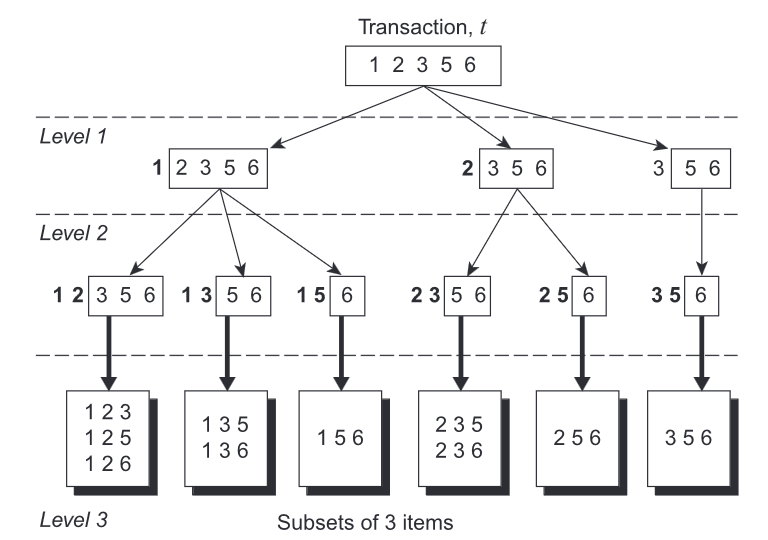
\includegraphics[width=0.7\linewidth]{img/apriori_prefixtree.png}   
\end{figure}

\section{Rule Generation}

Each frequent $k$-itemset, $Y$, can produce up to $2^k - 2$ association rules, excluding rules with empty antecedents or consequents. An association rule can be extracted by partitioning the itemset $Y$ into two non empty subsets, $X$ and $Y-X$, such that $c(X \rightarrow Y_X)$ is greater than \textit{minconf}. Computing the confidence of an association rule does not require additional scans of the transaction dataset. The itemsets from which rules are extracted from are all frequent, and so are their subsets.

Below is the pseudocode of the algorithm.

\begin{algorithm}
\caption{Rule generation of the Apriori algorithm.}
\begin{algorithmic}[1]
    \State TODO
\end{algorithmic}
\end{algorithm}

TODO

\nocite{*}
\bibliographystyle{plain}
\clearpage\bibliography{bibliography}

\end{document}
